\documentclass[11pt, oneside]{article}    % use "amsart" instead of "article" for AMSLaTeX format
\usepackage{geometry}                % See geometry.pdf to learn the layout options. There are lots.
\geometry{letterpaper}                    % ... or a4paper or a5paper or ... 
%\geometry{landscape}                % Activate for rotated page geometry
%\usepackage[parfill]{parskip}    % Activate to begin paragraphs with an empty line rather than an indent
\usepackage{graphicx} % Use pdf, png, jpg, or eps§ with pdflatex; use eps in DVI mode
% TeX will automatically convert eps --> pdf in pdflatex 
\usepackage{amssymb}
\usepackage[T1]{fontenc}
\usepackage[utf8]{inputenc}
\usepackage{authblk}
\usepackage{amsmath} %amsthm, amssymb, amsfonts
\usepackage{subcaption}
\usepackage{float}
\usepackage{graphicx}

\title{  MODELING THE EFFECTS OF DRUGS OF ABUSE ON HIV INFECTIONS WITH TWO VIRAL SPECIES}
\author[1,3]{Peter M. Uhl}
\author[1,2,3]{Naveen K. Vaidya}
\affil[1]{Computational Science Research Center, San Diego State University, San Diego, CA}
\affil[2]{Department of Mathematics and Statistics, San Diego State University, San Diego, CA}
\affil[3]{Viral Information Institute, San Diego State University, San Diego, CA}
%\date{} % Activate to display a given date or no date

\begin{document}
\maketitle
%\section{}
%\subsection{}

\begin{abstract}

Injection drug use is one of the greatest risk factors associated with contracting human immunodeficiency virus (HIV), and drug users infected with HIV suffer from a higher viral load and rapid pathogenesis. While replication of HIV may result in a large number of mutant viruses that can escape recognition of the host's immune response, the presence of morphine can decrease the viral mutation rate and cellular immune responses. In this study, we develop a mathematical model to study the effects of the decrease in mutation and cellular immune response in the presence of morphine on the viral dynamics. We consider two viral populations: a wild-type and a mutant. Our model predicts that the morphine-altered mutation rate and cellular immune response allow the wild-type virus to out compete the mutant virus, resulting in a higher set point viral load. We also compute the basic reproduction numbers and show that the dominant species is determined by a threshold morphine concentration, with the mutant dominating below and the wild-type dominating above the threshold. Furthermore, we identified three biologically relevant equilibria- the infection-free, mutant only, and coexistence equilibria- which can be completely characterized by fitness cost of mutation, mutant escape rate, and morphine concentration.

\end{abstract}

\section{Introduction}

	Human immunodeficiency virus (HIV) is a significant health concern around the world, with $36.9$ infected people worldwide in 2018 \cite{unaids}. In addtion to the sexual route, HIV transmission is also commonly associated with recreational drug use through needle sharing between drug users \cite{Alcabes}. Drug use has also been shown to have a number of detrimental effects in people infected with HIV, such as a higher viral load, a more rapid progression to AIDS, a greater chance of AIDS related neurological complications, and an overall higher mortality rate \cite{Kohli, Kumar, Hauser, Li}. It is therefore important to understand how conditioning of drugs of abuse affect the progression of HIV infections. 

\vspace{5mm}
	
	HIV replicates within target CD4+ T-cells. Individual virions bind to the target cell membrane, enter the nucleus of the target cell, replicate viral RNA, and then the now infected cell releases newly produced virus into the environment \cite{Kitchen,Killeen, Chan}. One of the defense mechanisms the host implements is a cellular immune response in the form of cytotoxic T-lymphocytes (CTLs), which are able to detect and kill infected cells by recognizing epitopes on the surface of infected cells, thereby limiting viral replication \cite{ Greenough, Ganusov2013}. The virus replication process is very error-prone, which results in a large number of mutations taking place \cite{Klein}. This results in a high number of mutant viruses that express epitopes different from the wild-type virus and escape detection by CTLs \cite{Klein, Fryer, Chan}. Pressure to escape CTLs, combined with the high turnover of virions and infected cells, plays a significant role in allowing HIV to establish infection \cite{Boutwell,McMichael,Ribeiro} and poses a major challenge in the control of the infection by immune responses, thereby causing obstacles in developing successful CTL-bases vaccines \cite{Deng, Konrad, Barouch}. 

\vspace{5mm}

	Animal models of SIV in rhesus macaques have demonstrated a number of adverse effects that drugs of abuse can have on the prognosis of an infection. In the experiment by Kumar et al \cite{Kumar}, morphine addicted animals were found to have decreased CD4+ T-cells and increased set-point viral load compared to non-addicted animals. A partial explanation for these results is that there are also evidences that morphine alters the evolution of SIV, lowering the viral diversity \cite{ Noel2006, Noel2007, Rivera-Amill}. Drugs of abuse have been shown to increase expression of the CC5R co-receptor in target cells, making them more susceptible to infection \cite{Kumar, Miyagi, Li} and opiates are also known to adversely affect the immune system \cite{Rivera-Amill}. Therefore, the potential alteration in mutation and immune response due to drugs of abuse needs to be considered to quantify the effects of opiate use on HIV infections.

\vspace{5mm}

Mathematical models have been used extensively to study infections diseases, including HIV/SIV \cite{Perelson, Chubb, Konrad, Conway, Schwartz, Vaidya, Mutua, Ganusov2006, Ganusov2011, Ganusov2013}. Previously, models have been developed to investigate viral escape \cite{Ganusov2006, Ganusov2011, Ganusov2013}, antibody responses \cite{Mutua}, and viral evolution\cite{Konrad}. In this study, we present a mathematical model of HIV infections that incorporates morphine effects on the dynamics of viral replication, cellular immune responses, and mutation. We analyze the model to determine how morphine use affects viral evolution and the long-term viral dynamics with mutant and wild-type (founder) virus species. We are able to fully characterize the dynamics using three steady state solutions of the model: an infection-free steady state, a mutant only steady state, and a coexistence steady state. Further, we are able to show that the stable steady state of the system can be determined by the concentration of morphine present in the body.

%and one of the most common forms of transmission is by sharing needles used for injecting drugs of abuse, such as opioids, between infected and non-infected persons. Drugs of abuse have been shown to have adverse effects on the progression of HIV infections, including a higher set point viral load and decreased amounts of CD4+ T cells \cite{Kumar}. Studies involving rhesus macaques and simian and human-simian immunodeficiency virus (SIV and HSIV) have shown that morphine may cause a faster progression to AIDS and pathogenesis in infected animals, and other studies of HIV have also demonstrated that a quicker progression to AIDS may be associated with opiate use \cite{Hauser}. It is therefore important to investigate the mechanisms by which morphine affects the progression of HIV infections and viral burden.

\vspace{5mm}

	%Cytotoxic T-lymphocytes (CTLs) are an important component of the human immune system for combating viral infections, including HIV, by limiting viral reproduction and the infection of hosts’ target cells. In the acute stage of the infection the host’s immune system responds by creating a large amount of virus specific CTLs. The CTLs perform actions to inhibit viral growth, for example by destroying infected cells directly. After the infection has progressed and the CTL immune response has been reduced it is possible for viruses to revert back to the original level (NEED REF). Therefore the production of CTLs plays a significant role in the progression of an infection \cite{Greenough}. Also, HIV possesses a high genetic variability which may result in the production of escape mutants that can avoid detection by CTLs \cite{Boutwell}. The high number of CTLs puts pressure on the virus to quickly mutate to a form that can evade the CTLs. This pressure, combined with the quick replication speed of HIV, may result in a large number of mutant viruses being produced \cite{Deng, Ribeiro}. The production of mutant viruses can be a significant barrier to the treatment of HIV by antiviral drugs or to the development of an effective vaccine \cite{Boutwell}.
	

\section{Methods}

\subsection{Mathematical Model}

\subsubsection{Virus-Cell Dynamics}

Our model is developed by extending a standard HIV dynamics model \cite{Perelson, Schwartz} to include morphine effects on target cell susceptibility, viral evolution, and cellular immune response. Following Vaidya et al. \cite{Vaidya, Mutua}, we include two populations of CD4+ target cells based on CCR5 co-receptor expression: a population with lower susceptibility to infection, $T_l$, and a population with higher susceptibility to infection, $T_h$, due to lower and higher levels of co-receptor expression, respectively \cite{Kumar, Miyagi,Li}. Viral mutation is modeled by including two viral species, a wild-type virus, $V_w$,  and a mutant virus, $V_m$, \cite{Klein, McMichael}. We assume free virus particles infect target cells to produce corresponding infected cell populations $I_w$ and $I_m$.  Cellular immune responses are represented by a population of CTLs, denoted $C$, which act by directly killing infected cells \cite{Konrad, De Boer}. 

%** 
% $F$ denotes the fitness cost of mutation, giving $F$ such that $0 \leqslant F \leqslant 1$. We assume that the mutant virus does not have a higher infection rate than the wild-type virus \cite{Ganusov2011}. 

%*** 
%Due to mutation,  a fraction $\epsilon$ of target cells infected by wild-type virus become mutant infected cells and the remainder, $(1-\epsilon)$, remain as wild-type infected cells \cite{Konrad}.

%****
%The mutant escape rate, $B > 0$, is a reduction in the ability of the host's cellular immune response to kill cells infected by the mutant virus compared to cells infected by the wild-type virus. Due to responses by epitope-specific CTLs there is some recognition of mutant infected cells by the host's immune responses \cite{Konrad, Barouch} and we interpret the escape rate as a rate of escape averaged over the entire mutant population. 

\vspace{5mm}

	Target cells are recruited at constant rate $\lambda$ and we assume that newly recruited cells all belong to the $T_l$ population. Target cells switch from $T_l$ to $T_h$ at rate $r$ and from $T_h$ to $T_l$ at rate $q$ \cite{Vaidya}. Both populations of target cells die at per capita rate $\delta_T$ \cite{Perelson, Schwartz}. Target cells in the $T_l$ population are infected by the wild-type virus at rate $\beta_l$ and by the mutant virus at rate $(1-F) \beta_l$, where $F$ denotes the fitness cost of mutation, giving $F$ such that $0 \leqslant F \leqslant 1$. We assume that the mutant virus does not have a higher infection rate than the wild-type virus \cite{Ganusov2011}. Similarly, $T_h$ cells are infected at rates $\beta_h$ and $(1-F) \beta_h$ by the wild-type and mutant viruses, respectively. Due to mutation,  a fraction $\epsilon$ of target cells infected by wild-type virus become mutant infected cells and the remainder, $(1-\epsilon)$, remain as wild-type infected cells \cite{Konrad}.

\vspace{5mm}
	
	Both virus species are produced by their corresponding infected cell population at rate $p$ per cell and are cleared at rate $\delta_V$ \cite{Konrad}. Mutant virus infects $T_l$ and $T_h$ cells at rates $(1-F) \beta_l$ and $(1-F) \beta_h$, respectively. We assume only forward mutation takes place, i.e., target cells infected by mutant virus will not revert to the wild-type infected population. Wild-type infected cells $I_w$ are killed by CTLs at rate $b$. CTLs kill $I_m$ cells at rate $\frac{b}{1+B}$, in which the base CTL killing rate $b$ is reduced by the mutant escape ratio $1+B$. The mutant escape rate, $B > 0$, is a reduction in the ability of the host's cellular immune response to kill cells infected by the mutant virus compared to cells infected by the wild-type virus. Due to responses by epitope-specific CTLs there is some recognition of mutant infected cells by the host's immune responses \cite{Konrad, Barouch} and we interpret the escape rate as a rate of escape averaged over the entire mutant population. Both classes of infected cells die at per capita rate $\delta_I$. CTLs are recruited at constant rate $\omega$ \cite{Conway}, die at rate $\delta_C$, and are also produced at rate $\alpha$ per infected cell, i.e., $I_w + I_m$ \cite{Konrad, De Boer}.

\vspace{5mm}

\subsubsection{Effects of Morphine}

	Based on experimental results, we include the effects of morphine through three mechanisms: the higher transfer of $T_l$ cells into $T_h$ cells due to increased co-receptor expression \cite{Kumar, Miyagi}, the decrease in viral evolution \cite{Noel2006, Noel2007}, and the decrease in CTL production \cite{Rivera-Amill}. We therefore make the transition parameters $r$ and $q$ morphine dependent, i.e., $r=r(M)$ and $q=q(M)$, where $M$ is the concentration of morphine. Since it is expected that $r(M)$ is an increasing function of morphine and $q(M)$ is a decreasing function of morphine (some ref here), we model $r(M)$ and $q(M)$ using an $E_{max}$ model of the form

\begin{align*}
r(M) &= r_c + (r_m - r_c) \eta_r(M),\\
q(M) &= q_m + (q_c - q_m) \eta_q (M),\\
\end{align*}

where 

\begin{align*}
\eta_r(M) &= \frac{M^n}{M_h^n + M^n},\\
\eta_q(M) &= 1- \eta_r(M).\\
\end{align*}

Here, $r_c$  and $r_m$ are the minimum and maximum values of $r(M)$, $q_c$ and $q_m$ are the minimum and maximum values of $q(M)$, $n$ is the Hill's coefficient for the $E_{max}$ model, and $M_h$ is the morphine concentration that gives $r(M)$ and $q(M)$ the value half-way between their respective minimums and maximums. Since morphine causes a decrease in viral mutation \cite{Noel2006,Noel2007}, we model the mutation rate as $\frac{\epsilon}{\mu + \eta M}$, where $\mu,\eta$ are parameters related to the effect of morphine on mutation. To model the decrease in CTL production due to morphine, we take the CTL recruitment rate as $\omega e^{-\psi M}$ and the CTL production rate in response to infection as $\frac{\alpha}{\gamma + \xi M}$, where $\psi, \gamma,\xi$ are parameters related to the decrease in CTL production due to morphine.

%by introducing parameters $\gamma,\xi$ and modeling the morphine dependent CTL production rate as $\frac{\alpha}{\gamma + \xi M}$. Finally, we assume the base CTL production rate, $\omega$, decreases exponentially with morphine with decay rate $\psi$, giving $\omega e^{-\psi M}$. To simplify notation we will sometimes write $\hat{\epsilon} = \frac{\epsilon}{\mu + \eta M}, \hat{\alpha} = \frac{\alpha}{\gamma + \xi M}$, and $\hat{\omega}= \omega e^{-\psi M}$.

\vspace{5mm}

	The full model is given by the following seven-dimensional system of ODE's:
\begin{align*}
%\frac{d T_l}{dt} & =  \lambda + q(M) T_h - r(M) T_l - \beta_l V_w T_l - (1-F) \beta_l V_m T_l - \delta_T T_l\\
\frac{d T_l}{dt} & =  \lambda + \left(q_m + (q_c - q_m) \left(1- \frac{M^n}{M_h^n + M^n}\right) \right) T_h - \left(r_c + (r_m - r_c) \frac{M^n}{M_h^n + M^n} \right)T_l \\
 	&  - \beta_l V_w T_l - (1-F) \beta_l V_m T_l - \delta_T T_l\\
\frac{d T_h}{dt}  & =  \left(r_c + (r_m - r_c) \frac{M^n}{M_h^n + M^n} \right) T_l -  \left(q_m + (q_c - q_m) \left(1- \frac{M^n}{M_h^n + M^n}\right) \right) T_h \\
	& - \beta_h V_w T_h - (1-F) \beta_h V_m T_h - \delta_T T_h\\
\frac{d V_w}{dt}  & =  p I_w - \delta_V V_w \\
\frac{d V_m}{dt} & =  p I_m - \delta_V V_m \\
\frac{d I_w}{dt} & =  (1-\frac{\epsilon}{\mu + \eta M})(\beta_l V_w T_l + \beta_h V_w T_h) - b I_w C - \delta_I I_w \\
\frac{d I_m}{dt} & = \frac{\epsilon}{\mu + \eta M}(\beta_l V_w T_l + \beta_h V_w T_h) + (1-F) (\beta_l V_m T_l +\beta_h V_m T_h) -\frac{b} {1+B} I_m C -\delta_I I_m\\
\frac{d C}{dt} & =  \omega e^{-\psi M} + \frac{\alpha}{\gamma + \xi M}(I_w + I_m)C - \delta_C C.\\
\end{align*}

\subsection{Parameter Estimation}

	We estimates parameter values based on previously published studies. Following Vaidya et al. \cite{Vaidya}, we assume $10^6$ target cells per $ml$ of blood,  with $40980/ml$ belonging to the $T_h$ population and the remaining $959020/ml$ to the $T_l$ population. We assume that the infection begins with only free virus and no infected cells, so we take $I_w(0),I_m(0) = 0$. Also, as described in Vaidya et al. \cite{Vaidya}, the SIV infection was established with $10^5$ RNA copies of the virus. Assuming a macaque contains approximately 1.5 liters of extracellular water we can estimate $V_0 = \frac{3\times 10^5 }{1.5 L} \approx 200$ viral RNA copies/ml \cite{Vaidya}, which we assume to belong entirely to the $V_w$ population. Estimates for $\lambda, \beta_l, \beta_h, r_c, r_m, q_m, q_c$, and $\delta_I$ were taken from Vaidya et al. \cite{Vaidya}, where these values were obtained by fitting the model to experimental data. In particular, they estimated $\beta_h$ as approximately two orders of magnitude higher than $\beta_l$. The viral production rate, $p$, is estimated from the SIV \textit{in vivo} burst size in rhesus macaques and the average life-span of an infected cell, giving $p=2500$ per cell/day \cite{Vaidya}.


\vspace{5mm}

 Based on modeling work by Stafford et al.\cite{Stafford}, we take $\delta_T = 1/100 = 0.01$, which corresponds to a target cell life span of 100 days. Ramratnam et al.\cite{Ramratnam} give an estimated range of HIV viral clearance between $9.1$ and $36$ virions per day, so we use their average value of 23 virions per day as our value for $\delta_V$. Mansky and Temin \cite{Mansky} determined the $in$ $vivo$ mutation rate of HIV-1 to be $3.4 \times 10^{-5}$ mutations per base pair per generation, so we take the mutation rate $\epsilon= 3 \times 10^{-5}$. Following De Boer and Perelson \cite{De Boer}, we take $\delta_C = 0.2$ as an estimate for the turnover of CTLs and $\frac{\alpha}{\gamma} = 6.7 \times 10^{-5}$ for the infected cell dependent CTL production rate . The value $\omega = 15$ was chosen to give a sufficiently large steady-state value for $C$.

\vspace{5mm}

Previous modeling work by Ganusov et al.\cite{Ganusov2011} investigated the rate of escape by mutant viruses from CTL responses. They measured the rate of escape by a single mutant variant as the average difference between the rate of mutant killing by CTLs and the production rate of the mutant. They consider a range of killing of infected cells (wild-type and mutant) by CTLs of 0.01-0.5 $day^{-1}$, so we take an intermediate value of $b=0.25$ $day^{-1}$ as our base value. In their study, the upper value $b = 0.5$ corresponds to a wild-type virus and the lower value $b = 0.01$ to an escape mutant. Noting that $\frac{0.5}{0.01} = 50$, we will vary the escape ratio, $1+B$, from $0-50$ with $B = 30$ as our base value \cite{Ganusov2011}.

% In addition, we will vary the fitness cost of mutation, $F$, between 0 and 1, noting that $F=0$ corresponds to a mutant that is as effective as the wild-type at infecting target cells while $F=1$ corresponds to a mutant that is not able to infect target cells at all.

\vspace{5mm}

	In an experiment performed in children aged between two and six years old, Olkkola et al. \cite{Olkkola} observed initial morphine concentrations between 28 and 198 $\mu g/l$ of blood plasma. To include this range, we will consider values of $M$ to be between 0 and 200  $\mu g/l$ \cite{Olkkola}. Accordingly, we take $M_h=100$ corresponding to the half-way value of $r(M)$ and $q(M)$.

\vspace{5mm}

	The estimated parameters and their descriptions are summarized in Table 1:

\begin{table}[H]
%\tiny
\centering
\caption{Parameter Values}
\vspace{3mm}
\begin{tabular}{|c|c|c|c|}
\hline
Parameter & Value & Description & Reference\\
\hline
$\lambda$ & 3690 $ml$ $day^{-1}$ & Production rate of $T_l$ cells & \cite{Vaidya}\\
\hline
$r_c$ & $0.16$ $day^{-1}$& Minimum value of $r$ &  \cite{Vaidya}\\
\hline
$r_m$ & $0.52$ $day^{-1}$ & Maximum value of $r$ & \cite{Vaidya}\\
\hline
$q_c$ & $1.23 \times 10^{-6}$  $day^{-1}$ & Minimum value of $q$ & \cite{Vaidya}\\
\hline
$q_m$ & $0.25$ $day^{-1}$ & Maximum value of $q$ & \cite{Vaidya}\\
\hline
$M_h$ & $100$ &  Half morphine value for $r(M),q(M)$  & \cite{Olkkola} \\
\hline
$n$ & $8$ &  Hill's coefficient of morphine response  & --\\
\hline
$\beta_l$ & $10^{-9} ml$ $day^{-1}$ & Wild- type infection rate of $T_l$ cells & \cite{Vaidya}\\
\hline
$\beta_h$ & $10^{-7} ml$ $day^{-1}$ & Wild -type infection rate of $T_h$ cells & \cite{Vaidya} \\
\hline
$F$ & $0.1$ & Fitness cost of mutation & --\\
\hline
$p$ & $2500$ $day^{-1}$ & Production rate of virus & \cite{Vaidya} \\
\hline
$b$ & $0.25$ $ml$ $day^{-1}$ & CTL killing rate of wild-type & \cite{Ganusov2011}\\
\hline
$B$ & $30$ & Mutant escape ratio & --\\
\hline 
$\alpha$ & $6.7 \times 10^{-5}$ $ml$ $day^{-1}$ & CTL response to infection & \cite{De Boer}\\
\hline
$\gamma$ & $1$ & Morphine effect on $\alpha$ & --\\
\hline
$\xi$ & $1$ $l$ $\mu g ^{-1}$ & Morphine effect on $\alpha$ & --\\
\hline
$\omega$ & $15$ $ml$ $day^{-1}$  & Base CTL production rate & --\\
\hline
$\psi$ & $0.1$ & CTL prduction decay rate & --\\
\hline
$\epsilon$ & $3 \times 10^{-5}$ & Mutation rate & \cite{Mansky}\\
\hline
$\mu$ & $1$ & Morphine effect on $\epsilon$ & --\\
\hline
$\eta$ & $1$ $l$ $\mu g ^{-1}$ & Morphine effect on $\epsilon$ & -- \\
\hline
$\delta_T$ & 0.01 day$^{-1}$ & Target cell death rate & \cite{Stafford} \\
\hline
$\delta_V$ & 23 day$^{-1}$ & Virus clearance rate & \cite{Ramratnam} \\
\hline
$\delta_I$ & 0.7 day$^{-1}$ & Infected cell death rate & \cite{Vaidya}\\
\hline
$\delta_C$ & 0.2 day$^{-1}$ & CTL death rate & \cite{De Boer}\\
\hline
$M$ & $0-200$ $\mu g$ $l^{-1}$ & Concentration of morphine & \cite{Olkkola}\\
\hline
\end{tabular}
\end{table}


\section{Results}
\subsection{Basic Reproduction Number}
\subsubsection{Derivation and Sensitivity}

The basic reproduction number, denoted by $R_0$, is an important quantity in the study of viral dynamics and is defined as the average number of secondary infected cells resulting from a single initial infected cell when target cells are not limited \cite{Castillo-Chavez}. $R_0$ provides a threshold condition for infection to persist ($R_0 > 1$) and to die out ($R_0 < 1$).

%The stability of the infection free equilibrium (IFE) can be described by the basic reproduction number, with the IFE being locally asymptotically stable if $R_0 < 1$ and unstable if $R_0 >1$ \cite{Castillo-Chavez}. Since our model contains two viral species, the basic reproduction number is obtained, as we show below, as a combination of the quantities $R_0^w$ and $R_0^m$, corresponding to the wild-type and mutant viruses, respectively. 

\vspace{5mm}

	 We use the next generation matrix method \cite{Diekmann} to obtain an expression for the basic reproduction number of our model. The next-generation matrix is obtained from the infected subsystem of the model, i.e., the equations of the system corresponding to viruses and infected cells \cite{Diekmann}. For our model, the infected subsystem is given by

%\vspace{10mm}

\begin{align*}
\frac{d V_w}{dt} & =  p I_w - \delta_V V_w\\
\frac{d V_m}{dt} & =  p I_m - \delta_V V_m\\
\frac{d I_w}{dt} & =  (1-\hat{\epsilon}(M))(\beta_l V_w T_l + \beta_h V_w T_h) - b I_w C - \delta_I I_w\\
\frac{d I_m}{dt} & =  \hat{\epsilon}(M)(\beta_l V_w T_l + \beta_h V_w T_h) +  (\hat{\beta_l} V_m T_l +\hat{\beta_h} V_m T_h)  -\frac{b}{1+B} I_m C -\delta_I I_m,\\
\end{align*}


where $\hat{\epsilon}(M) =  \frac{\epsilon}{\mu + \eta M}$, $\hat{\beta_l} = (1-F) \beta_l$, and $\hat{\beta_h} = (1-F) \beta_h$. The infection free equilibrium (IFE) is the steady-state solution of the model in which all infected populations are zero. For our model, we compute the IFE as $(T_l^*,T_h^*,0,0,0,0,C^*)$, where

\begin{align*}
T_l^* & =  \frac{\lambda (q(M) + \delta_T)}{\delta_T (q(M) + r(M) +\delta_T)},\\
T_h^* & =  \frac{\lambda r(M)}{\delta_T (q(M) + r(M) +\delta_T)},\\
C^* & = 	 \frac{\hat{\omega}(M)}{\delta_C},\\
\end{align*}

\hspace{-7mm} and $\hat{\omega}(M) = \omega e^{-\psi M}$. Now, we linearize the infected subsystem about the IFE and decompose it into $\mathcal F - \mathcal V$, where $\mathcal F$ is the infection part of the system, which describes newly infected components, and $\mathcal V$ is the transition part, which describes transitions of cells and viruses in and out of compartments.  $\mathcal F$ and $\mathcal V$  for our model are given by

\vspace{5mm}

\begin{align*}
{\mathcal F} & =  \begin{bmatrix}
 0 & 0 & 0 & 0\\
0 & 0 & 0 & 0\\
(1-\hat{\epsilon}(M)) ( \beta_l T_l^* + \beta_h T_h^*) & 0 & 0 & 0\\
\hat{\epsilon}(M) ( \beta_l T_l^* + \beta_h T_h^*) & (\hat{\beta_l} T_l^* + \hat{ \beta_h} T_h^*) & 0 & 0\\
\end{bmatrix}
\end{align*}

and 

\begin{align*}
{\mathcal V} & =  \begin{bmatrix}
\delta_V & 0 & -p & 0\\
0 & \delta_V & 0 & -p\\
0 & 0 & \delta_I + b C^* & 0\\
0 & 0 & 0 & \delta_I + \frac{b}{1+B} C^*\\
\end{bmatrix}.
\end{align*}

\vspace{5mm}

The next generation matrix is ${\mathcal F \mathcal V}^{-1}$ and its spectral radius $\rho(\mathcal F \mathcal V^{-1})$ is the basic reproduction number of the system \cite{Diekmann}. The basic reproduction number of our model is thus obtained as $R_0 = \sigma(\mathcal F \mathcal V^{-1}) = \max\{R_0^w,R_0^m\}$, where 

\begin{align*}
R_0^w & = \frac{(1 - \hat{\epsilon}(M)) (\beta_h T_h^* +  \beta_l T_l^*)p}{\delta_V (bC^* + \delta_I)},\\
R_0^m &= \frac{(1-F)(\beta_h T_h^* +  \beta_l T_l^*)(1+B)p}{\delta_V (\delta_I B + bC^* + \delta_I)},  \\
\end{align*}

represent the basic reproduction number corresponding to the wild-type and mutant virus, respectively. Note that since $\hat{\epsilon}(M), T_l^*, T_h^*$, and $C^*$ are morphine dependent, $R_0^w$ and $R_0^m$ are also morphine dependent. In addition, if $R_0^w, R_0^m <1$ the infection will die out while if either $R_0^w > 1$ or $R_0^m > 1$ the infection will be established \cite{Castillo-Chavez}. Using the parameter values in Table 1, we compute $R_0^w = 0.08$, $R_0^m = 1.07$, and $R_0 = max\{R_0^w,R_0^m\} = 1.07$, indicating the infections persists.

\vspace{5mm}

To study the effect of each parameter on the value of $R_0$, we determine how sensitive $R_0^w$ and $R_0^m$ are to changes in individual parameters. For a parameter $\rho$ of the model, the forward sensitivity index is given by 

\begin{align*}
S_\rho & = \frac{\rho}{R_0}\frac{\partial R_0}{\partial \rho}.
\end{align*}

Then $S_{\rho}$ determines the relative change in $R_0$ caused by a change in $\rho$ \cite{Marino, Perera, Rodrigues}. The higher the values of $S_\rho$, the more sensitive $R_0$ is to $\rho$. Also, positive (negative) values of $S_{\rho}$ indicate that $R_0$ increases (decreases) as $\rho$ increases. Sensitivity indices for $R_0^w$ and $R_0^m$ are shown in Figure~\ref{fig:sen_ind}; both quantities are strongly positively related to $\lambda, r, p,$ and $\delta_T$, indicating that increases in these parameters are favorable to the infection. Both quantities are also negatively related to $q, b, \delta_T,$ and $\omega$, indicating that increases in these parameters are unfavorable to the virus. In addition, $R_0^m$ is positively related to $B$ and negatively related to $F$.

\begin{figure*}[h]
    \centering
    \begin{subfigure}[b]{0.5\textwidth}
        \centering
        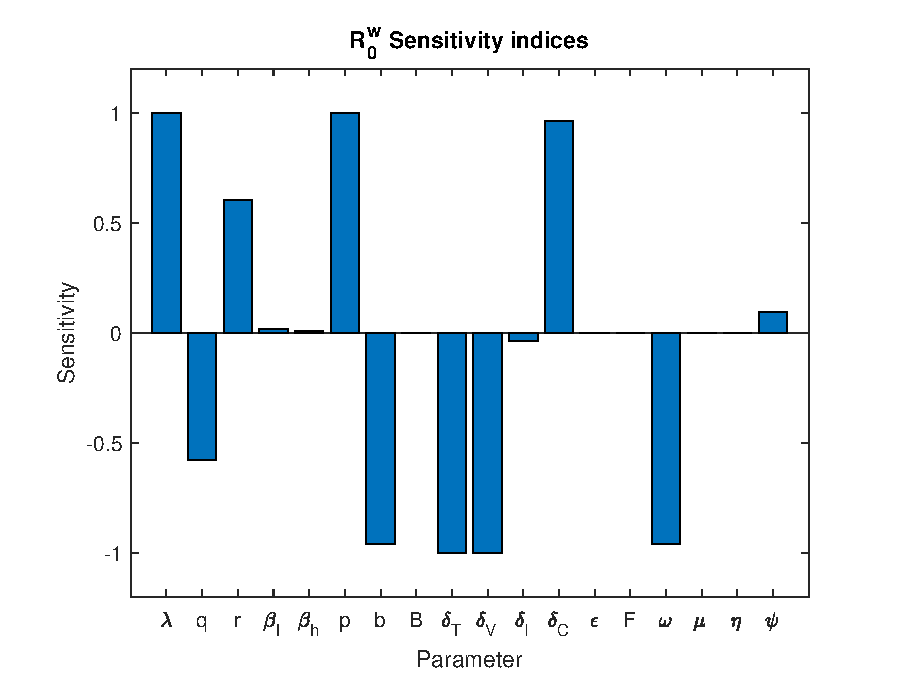
\includegraphics[scale=0.55]{rw_sen.eps}
        %\caption{$R_w^0$ sensitivity indices}
    \end{subfigure}%
    ~ 
    \begin{subfigure}[b]{0.5\textwidth}
        \centering
        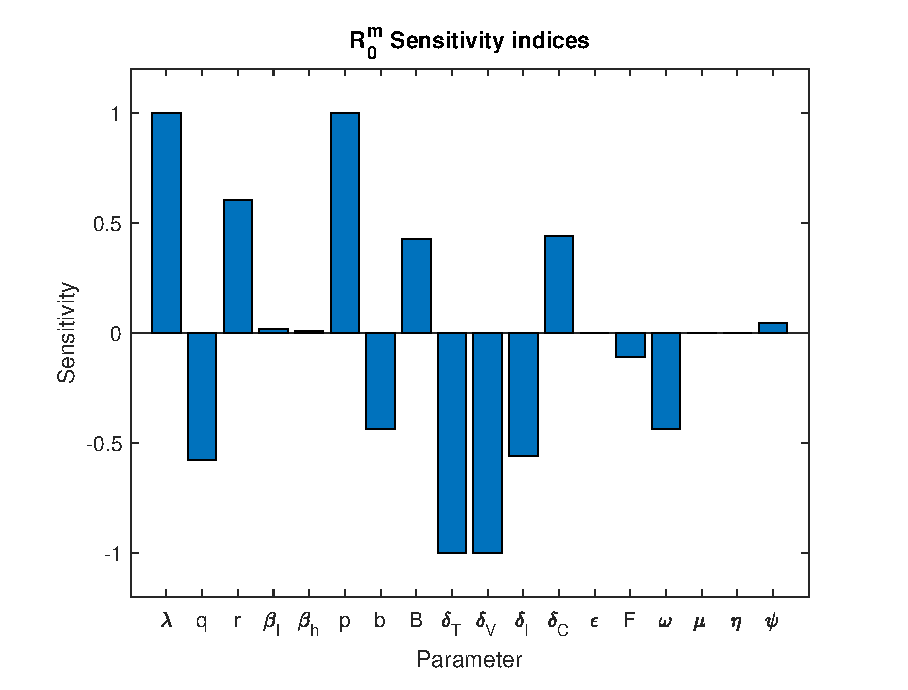
\includegraphics[scale=0.55]{rm_sen.eps}
        %\caption{$R_w^0$ sensitivity indices}
    \end{subfigure}
    \caption{Sensitivity indices for $R_0^w$ (left) and $R_0^m$ (right). A positive (negative) sensitivity index is favorable (unfavorable) to the virus. The higher the value of the sensitivity index, the more sensitive $R_0$ is to the parameter.}
\label{fig:sen_ind}
\end{figure*}

\subsubsection{Virus Species Switch}
\label{section:Virus Species Switch}

The viral species with a larger reproduction number is considered to be the dominant species. For the base case we obtained $R_0^w = 0.08$ and $R_0^m = 1.07$ indicating that the infection persists and the mutant is the dominant viral population when $M=0$. However, increasing the amount of morphine past a threshold value, $M_{thresh}$, results in a viral species switch where the wild-type becomes the viral dominant population. 

\begin{figure}[H]
\begin{center}
%\title{Basic Reproduction Number}
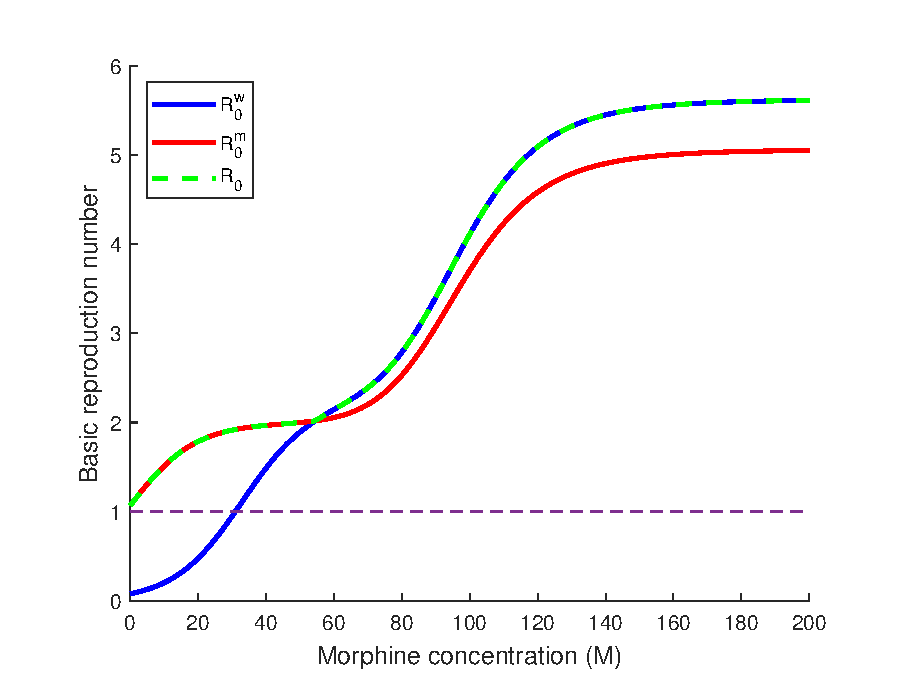
\includegraphics[scale=0.75]{pop_switch.eps}
\caption{$R_0^w$ and $R_0^m$ as functions of $M$. With parameter values as in Table 1, $M_{thresh} \approx 54$. The mutant is the dominant population for $M<54$ and the wild-type is dominant for $M>54$.}
\label{fig:pop_switch}
\end{center}
\end{figure}
% Figure~\ref{fig:pop_switch}

We can determine the value of $M_{thresh}$ by solving $R_0^w(M) = R_0^m(M)$ for $M$. If $M<M_{thresh}$ the mutant will dominate and if $M>M_{thresh}$ the wild-type will dominate. Due to the non-linear form of $R_0^w$ and $R_0^m$ we did not find a closed form for $M_{thresh}$, and obtained it numerically. For our base parameter values, $M_{thresh} \approx 54$, the wild-type is the dominant population for $M>54$ and the mutant dominates for $M<54$. Figure~\ref{fig:pop_switch} shows that as $M$ increases, the wild-type virus becomes the dominant species and for $M=200$ we have $R_0^w = 5.6$, $R_0^m = 5.05$.







\subsubsection{Effect of Fitness Cost and immune escape on $M_{thresh}$}

In this section we evaluate the effect of the values of $F$ and $B$ on $M_{thresh}$. $M_{thresh}$ is a decreasing function of $F$. As predicted by our model (Figure~\ref{fig:M_thresh_F_B}), $M_{thresh}$ decreases as $F$ increases. When the fitness cost is low, the mutant virus can out compete the wild-type virus for higher concentrations of morphine. For a very high fitness cost (for example $F>0.93$ in our computations), the mutant population is not fit enough to out compete the wild-type, which allows the wild-type to dominate for all values of $M$. In particular, if we take $F=1$ in the expression for $R_0^m$,

%Since there is uncertainty in the values of the fitness cost of mutation and mutant escape ratio, we wish to see how $M_{thesh}$ is affected by changing the values of $F$ and $B$. Figure~\ref{fig:M_thresh_F_B} shows $M_{thresh}$ as a function of $F$ and $B$. $M_{thresh}$ decreases as $F$ increases and we can only obtain a real value of $M_{thresh}$ for $ F < 0.933$. Low values of $F$ represent a low fitness cost and a mutant population that is nearly as fit as the wild-type. Therefore, when we have a very low fitness cost, the mutant is able to out compete the wild-type for higher concentrations of morphine. Alternatively, very high fitness costs ($F > 0.933$) corresponds to a mutant population that is not fit enough to out compete the wild-type even for very low morphine concentrations, which results in the wild-type dominating for all values of $M$. In particular, if we take $F = 1$ in the expression for $R_0^m$,

\begin{align*}
R_0^m &= \frac{(1-F)(\beta_h T_h^* +  \beta_l T_l^*)(1+B)p}{\delta_V (\delta_I B + bC^* + \delta_I)},  \\
\end{align*}

we obtain $R_0^m = 0$, implying that the mutant population is not reproducing.

\begin{figure*}[h]
    \centering
    \begin{subfigure}[b]{0.5\textwidth}
        \centering
        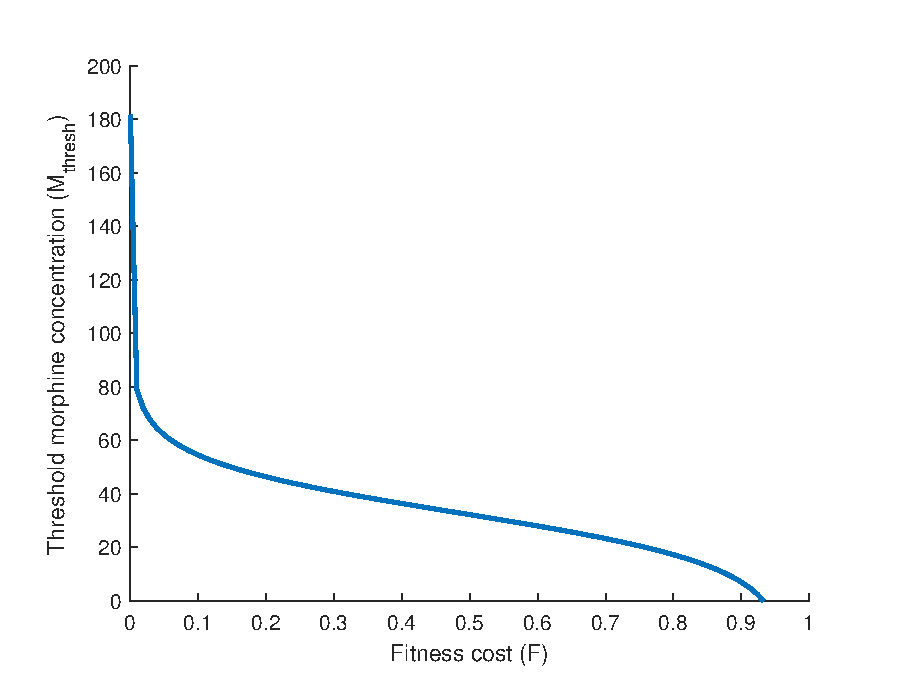
\includegraphics[scale=0.6]{M_thresh_F.eps}
        %\caption{$R_w^0$ sensitivity indices}
    \end{subfigure}%
    ~ 
    \begin{subfigure}[b]{0.5\textwidth}
        \centering
        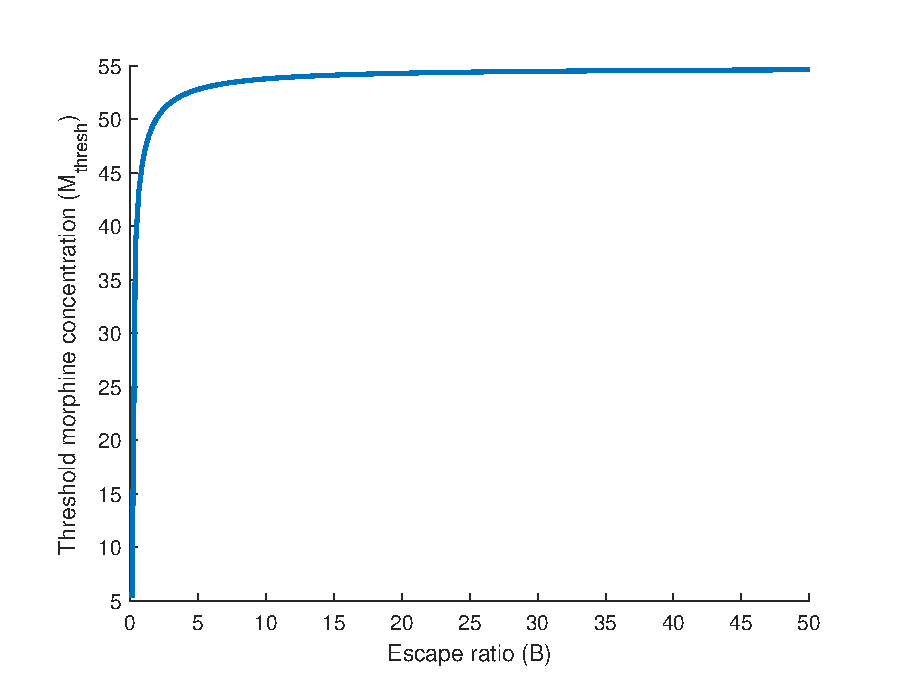
\includegraphics[scale=0.6]{M_thresh_B.eps}
        %\caption{$R_w^0$ sensitivity indices}
    \end{subfigure}
    \caption{(Left) $M_{thresh}$ as a function of $F$. For $F>0.93$, $M_{thresh}$ does not exist and the wild-type dominates for any value of $M$. (Right) $M_{thresh}$ increases as $B$ increases and saturates at approximately $B>5$. The wild-type always dominates for $B<0.12$.}
\label{fig:M_thresh_F_B}
\end{figure*}

	In our model, the escape ratio $B$ represents a reduction in the CTL killing rate of the mutant population compared to that of the wild-type population. The case $B=0$ corresponds to a mutant population that can be killed by CTLs as effectively as the wild-type population. For a low enough value of $B$ ($B<0.12$ for our base parameter values) we did not find any value of $M_{thresh}$. For a higher value of $B$ (i.e. $B>0.12$), $M_{thresh}$ increases as $B$ increases, i.e. the higher the escape ratio, the larger the morphine threshold for wild-type dominance will be (Figure~\ref{fig:M_thresh_F_B}).

 %i.e., $\frac{b}{1+B}$, so that increasing $B$ means fewer mutant infected cells are killed by CTLs. Similarly, $B=0$ corresponds to a mutant population that is killed by CTLs as readily as the wild-type population (in this case, $\frac{b}{1+B} = b$ so the killing rates are the same). Taking a low enough value of $B$ ($B \approx 0.255$ for our base parameter values) results in no real value of $M_{thresh}$ and the wild-type population dominating for all $M$.

\begin{figure}[H]
\begin{center}
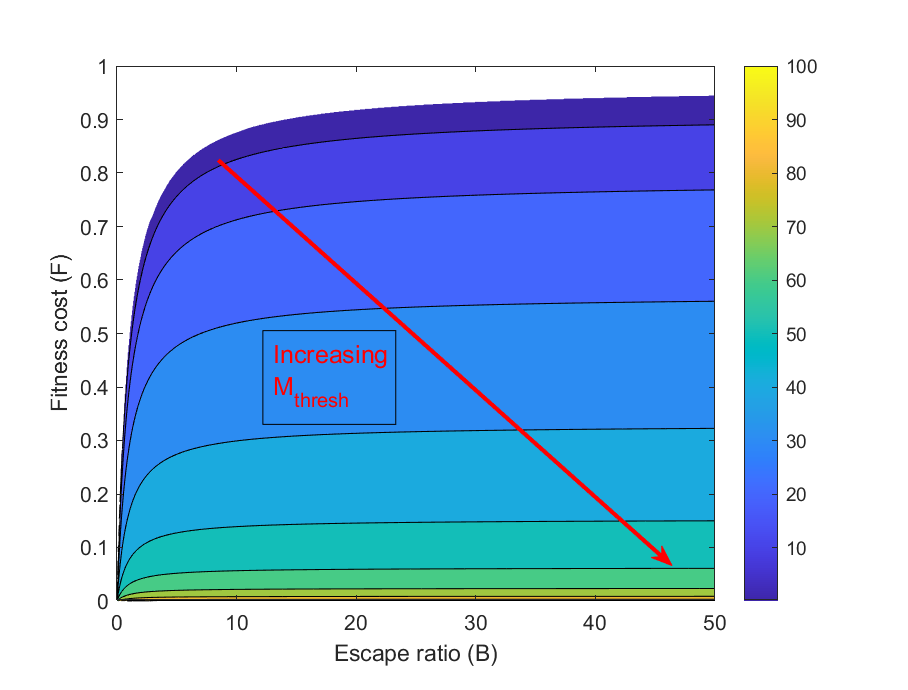
\includegraphics[scale=0.75]{FB_surf.eps}
\caption{$M_{thresh}$  in $F-B$ parameter space. The upper-left region represents $(F,B)$ values that cause the wild-type to always dominate. Moving along the arrow from the upper left corner to the lower right corner, the value of  $M_{thresh}$ increases.}
\label{fig:FB_surf}
\end{center}
\end{figure}

We also varied $F$ and $B$ simultaneously and computed $M_{thresh}$ as shown by the contour plot in $F-B$ parameter space (Figure~\ref{fig:FB_surf}). The upper-left unshaded region of the contour plot represents a combination of high fitness cost and low escape ratio that prevents the mutant population from out competing the wild-type. Increasing $F$ and decreasing $B$ lowers the threshold concentration of morphine required for wild-type virus to dominate  (Figure~\ref{fig:FB_surf}).

	

\subsection{Stability of steady-states}

\subsubsection{Infection Free Equilibrium (IFE)}

The IFE is shown in Section 3.1.1. As discussed earlier, the local stability of the IFE is determined by the basic reproduction number. It is easy to prove that the IFE is locally asymptotically stable if $R_0 < 1$ and unstable if $R_0 >1$ \cite{Castillo-Chavez}.

%Values of the quantities $R_0^w$ and $R_0^m$ are plotted in Figure 1, and $R_0 = \max\{R_0^w,R_0^m\}$ . The IFE is locally asymptotically stable if both $R_0^w$ and $R_0^m$ are less than one and unstable otherwise \cite{Castillo-Chavez}. We interpret this to mean that if the IFE is locally asymptotically stable then initial conditions near the IFE will converge to the IFE and the infection will not persist. If the IFE is unstable then initial conditions near the IFE will move away from it and infection will be established \cite{Perko, Jordan}. The dominant viral population is determined by the morphine concentration, with higher values favoring the wild-type virus and lower values favoring the mutant. 

\subsubsection{Mutant Only Equilibrium (MOE)}

The mutant only equilibrium (MOE) is the steady-state solution to the model in which there is no wild-type virus and only the mutant population exists. The MOE of our model takes the from $(\hat{T_l}, \hat{T_h},0,\hat{V_m},0,\hat{I_m},\hat{C})$, where

\begin{align*}
\hat{T_h} & = \frac{r(M) \lambda}{(q(M) + \hat{\beta_h} \hat{V}_m + \delta_T) ( r(M)+ \hat{\beta_l} \hat{V}_m + \delta_T) -r(M)q(M)}, \\
\hat{T_l} & = \frac{\lambda (q(M) + \hat{\beta_h} \hat{V}_m +\delta_T)}{(q(M) + \hat{\beta_h} \hat{V}_m + \delta_T) ( r(M)+ \hat{\beta_l} \hat{V}_m \delta_T) -r(M)q(M)}, \\
\hat{I_m} & = \frac{\delta_V \hat{V}_m}{p},\\
\hat{C} & = \frac{\hat{\omega}(M)}{\delta_C - \hat{\alpha} \frac{\delta_V \hat{V}_m}{p}}, \\
\end{align*}

and $\hat{V}_m$ is the solution to 

\begin{align}
g(\hat{V)}_m & = 0,
\end{align}

where

\begin{align*}
g(\hat{V_m}) & = \frac{\hat{\beta_l} \hat{V_m} \lambda \left(\hat{V_m} \hat{\beta_h} + q(M) + \delta_T \right) + \hat{\beta_h} r(M) \hat{V_m} \lambda   }   {\left(\hat{V_m} \hat{\beta_h} + q(M) + \delta_T \right)  
  \left(\hat{V_m} \hat{\beta_l} + r(M)+\delta_T \right) - r(M)q(M)} \\
 &	\quad  -  \frac{b \delta_V \hat{V_m} \hat{\omega}}{ \left(1+B\right) p \left( \delta_C - \frac{\hat{\alpha} \delta_V V_m^*}{p}  \right)  }      
- \frac{\delta_I \delta_V \hat{V_m}}{p} . \\
\end{align*}

Clearly, $\hat{V}_m = 0$ is a solution which corresponds to the IFE. We now desire a solution set with $\hat{V}_m > 0$. We obtain a value for $\hat{V_m}$ by solving (1) numerically, and compute values of $\hat{T_h},\hat{T_l},\hat{I_m},$ and $\hat{C}$.  $\hat{V_m}$ as a function of $M$ (Figure~\ref{fig:moe_vm} ) shows that increasing $M$ causes a larger non-zero equilibrium value of $\hat{V_m}$, indicating a higher set point viral load for larger morphine concentrations. Moreover, increasing $M$ reduces values of $T_l, T_h,$ and $C$ and increases the value of $I_m$ at the MOE (Figure~\ref{fig:other_MOEs}). From these we conclude that morphine causes more target cells to be infected and fewer infected cells to be killed by CTLs at the MOE.

\begin{figure*}[h]
    \centering
    \begin{subfigure}[b]{0.5\textwidth}
        \centering
        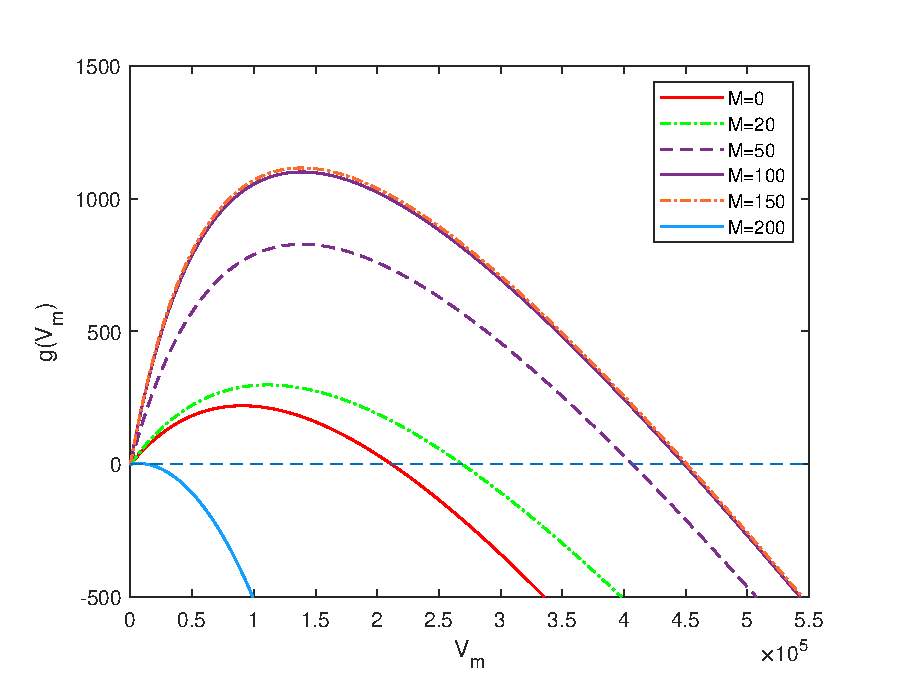
\includegraphics[scale=0.55]{some_vm_moes.eps}
        %\caption{$R_w^0$ sensitivity indices}
    \end{subfigure}%
    ~ 
    \begin{subfigure}[b]{0.5\textwidth}
        \centering
        \includegraphics[scale=0.55]{vm_moe_sim.eps}
        %\caption{$R_w^0$ sensitivity indices}
    \end{subfigure}
    \caption{$\hat{V}_m$ MOE values for different morphine concentrations. (Left) The positive zero-intercept of the curves are the $\hat{V}_m$ value for the particular value of $M$. (Right) Increasing $M$ gives a higher set point viral load of the MOE.}
\label{fig:moe_vm}
\end{figure*}

\begin{figure}[H]
\begin{center}
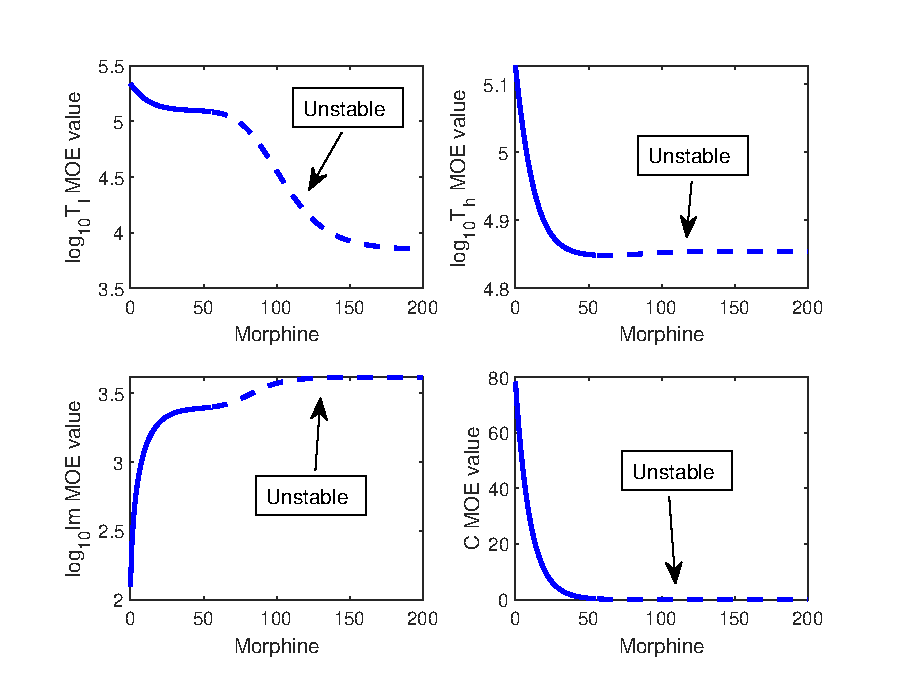
\includegraphics[scale=0.9]{other_MOEs.eps}
\caption{$T_l,T_h,I_m$, and $C$ values as functions of morphine. Morphine decreases the values of $T_l, T_h,$ and $C$ and increases the value of $I_m$ at the MOE.}
\label{fig:other_MOEs}
\end{center}
\end{figure}

%\subsubsection{Local Stability of the Mutant Only Equilibrium}

To determine the local stability of the MOE, we calculate the eigenvalues of the Jacobian matrix, $J$, of the model evaluated at the MOE, given by

\begin{align*}
J & = \begin{bmatrix}
J_{11} & J_{12} & J_{13} & J_{14} & 0 & 0 & 0\\
J_{21} & J_{22} & J_{23} & J_{24} & 0 & 0 & 0\\
0 & 0 & J_{33} & 0 & J_{35} & 0 & 0\\
0 & 0 & 0 & J_{44} & 0 & J_{46} & 0 \\
J_{51} & J_{52} & J_{53} & 0 &J_{55} & 0 &J_{57}\\
J_{61} &J_{62} & J_{63} & J_{64} & 0 &J_{66} &  J_{67}\\
0 & 0 & 0 & 0 & J_{75} & J_{76} &J_{77}\\
\end{bmatrix},
\end{align*}

where 

\begin{center}
$\begin{array}{rclrcl}
J_{11} & =&-r(M) - \beta_l V_w - \hat{\beta_l} V_m -\delta_T,                  &J_{52} & = &(1 - \hat{\epsilon}(M)) \beta_h V_w,  \\
 J_{12} & = & q(M),                            &J_{53} & = & (1 - \hat{\epsilon} (M))(\beta_l T_l + \beta_h T_h), \\
 J_{13} & = & -\beta_l T_l,                            &J_{55} & = &  -bC - \delta_I,  \\
 J_{14} & = &  -\hat{\beta_l} T_l,                         &J_{57} & = &  -b I_w,  \\
J_{21} & = & r(M),                     & J_{61} & = &\hat{\epsilon}(M) ( \beta_l V_w + \hat{\beta_l} V_m), \\
 J_{22} & = & -q(M)-\beta_h V_w - \hat{\beta_h} V_m -\delta_T,      & J_{62} & = &  \hat{\epsilon}(M)  \beta_h V_w + \hat{\beta_h} V_m, \\
J_{23} & = &  -\beta_h T_h,                    & J_{63} & = & \hat{\epsilon}(M) (\beta_l T_l + \beta_h T_h), \\
 J_{24}& = &  -\hat{\beta_h} T_h,                   & J_{64} & = &  \hat{\beta_l} T_l +\hat{\beta_h} T_h,     \\
J_{33} & = &-\delta_V,                   &J_{66} & = & -\frac{b}{1+B} C - \delta_I,  \\
J_{35} & = & p,                  &J_{67} & = &  -\frac{b}{1+B} I_m, \\
 J_{44} & = & -\delta_V,                &J_{75} & = & \hat{\alpha}(M)  C,  \\
 J_{46} &= & p,            &J_{76} & = &  \hat{\alpha}(M) C,   \\
J_{51} & = & (1 - \hat{\epsilon}) \beta_l V_w,               & J_{77} & = &  \hat{\alpha}(M)(I_w + I_m) - \delta_C.   \\
\end{array}$
\end{center}

 The MOE is locally asymptotically stable if the real part of each eigenvalue of $J$ is negative and unstable otherwise \cite{Perko,Jordan}. We now determine how $M$ affects the stability of the MOE.  The real parts of the seven eigenvalues of $J(MOE)$ for $0 \leq M \leq 200$ are shown in Figure~\ref{fig:MOE_eigs}. The real part of one of the eigenvalues becomes positive and the MOE becomes unstable for $M > 54$. This is consistent with the viral species switch seen in Section~\ref{section:Virus Species Switch} in which the larger values of $M$ allows the wild-type virus to dominate.

\vspace{5mm}

\begin{figure*}[h]
    \centering
    \begin{subfigure}[b]{0.5\textwidth}
        \centering
        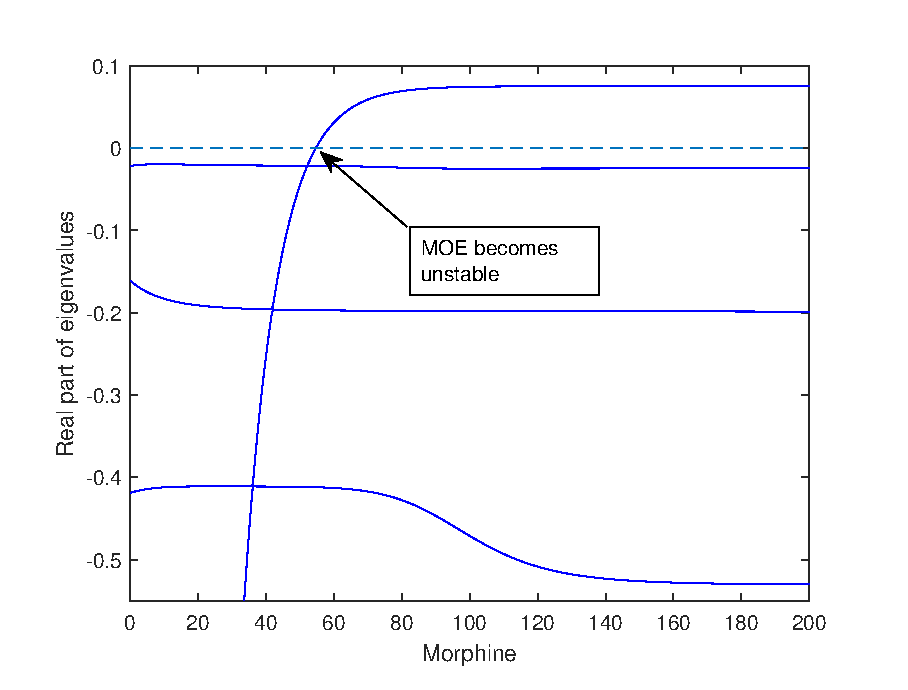
\includegraphics[scale=0.55]{MOE_some_eigs.eps}
        %\caption{$R_w^0$ sensitivity indices}
    \end{subfigure}%
    ~ 
    \begin{subfigure}[b]{0.5\textwidth}
        \centering
        \includegraphics[scale=0.55]{imag_parts.eps}
        %\caption{$R_w^0$ sensitivity indices}
    \end{subfigure}
    \caption{Eigenvalues of $J$ evaluated at the MOE. The figure on the left shows the four largest real parts. The right shows the imaginary parts of a pair of complex conjugate eigenvalues. The MOE becomes locally unstable near $M=54$.}
\label{fig:MOE_eigs}
\end{figure*}


\begin{figure*}[h]
    \centering
    \begin{subfigure}[b]{0.5\textwidth}
        \centering
        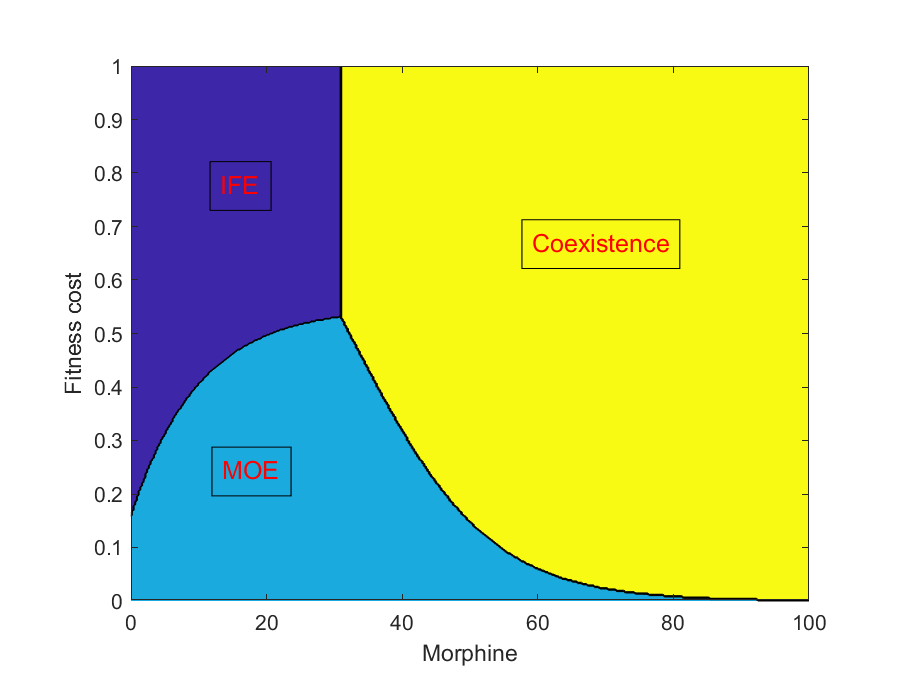
\includegraphics[scale=0.55]{MOE_F_contour.eps}
        %\caption{$R_w^0$ sensitivity indices}
    \end{subfigure}%
    ~ 
    \begin{subfigure}[b]{0.5\textwidth}
        \centering
        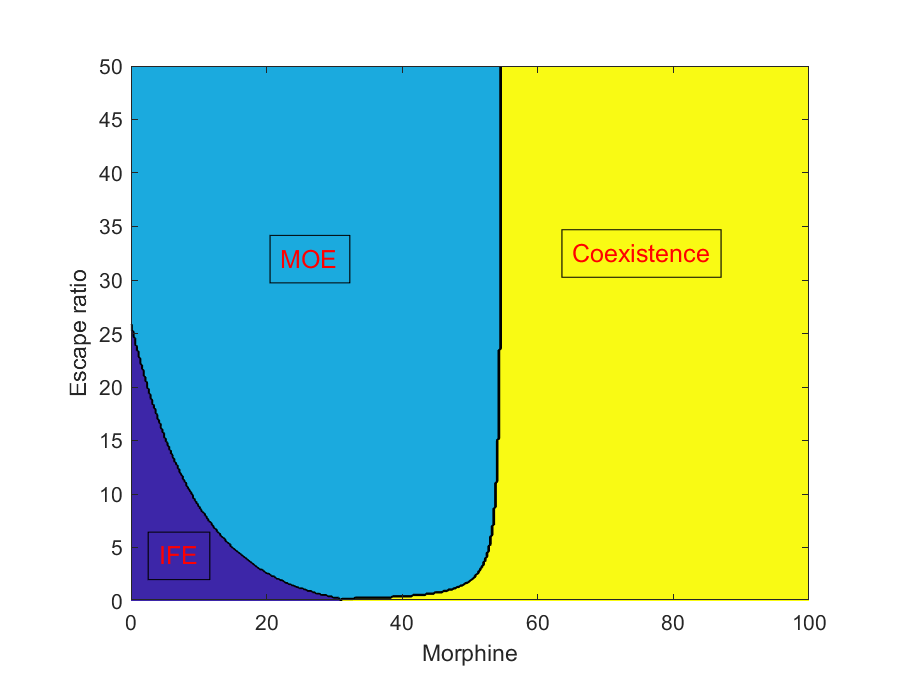
\includegraphics[scale=0.55]{MOE_B_contour.eps}
        %\caption{$R_w^0$ sensitivity indices}
    \end{subfigure}
    \caption{Stability regions in $M-F$ space (left, with $B = 30$) and $M-B$ space (right, with $F=0.1$). If $R_0^w,R_0^m < 1$ the system will evolve to the IFE. If the $R_0^m >1$ and $R_0^m >R_0^w$ the system will evolve to the MOE. Otherwise, the two viral species will coexist in a stable equilibrium.}
\label{fig:stab_regions}
\end{figure*}

We found that a bifurcation takes place at $R_0 = 1$ because the stability of the IFE changes at that point and we have shown that the parameters $F$ and $B$ affect the stability of the MOE. We can also show that for low $F$ and high $B$ the MOE does not exist and the IFE is the only stable equilibrium.  For values of $F$ and $B$ for which $R_0^m < 1$ the mutant population will not survive, hence $\hat{V}_m = 0,\hat{I}_m = 0$. It follows that

\begin{align*}
\hat{T}_h &= \frac{r(M) \lambda}{(q(M) + \delta_T) (r(M) + \delta_T) - r(M)q(M) }\\
 & = \frac{r(M) \lambda}{r(M)q(M) + q(M) \delta_T + r(M) \delta_T + \delta_T^2 - r(M)q(M)} \\
 & = \frac{r(M) \lambda}{ q(M) \delta_T + r(M) \delta_T + \delta_T^2 } \\
& = \frac{r(M) \lambda}{ \delta_T (q(M)  + r(M) + \delta_T) } \\
& = T_h^*, \\
\hat{T}_l & = \frac{r(M) \lambda}{\delta_T (q(M)  + r(M) + \delta_T)}  \frac{q(M) + \delta_T}{r(M)} \\
& = \frac{\lambda (q(M) + \delta_T)}{ \delta_T (q(M)  + r(M) + \delta_T) }  \\
& = T_l^*, \\
\hat{C} &= \frac{\hat{\omega}}{\delta_C} \\
& = C^*. \\
\end{align*}

Therefore, when $R_0^m < 1$ the MOE does not exist.

%We now observe the effects of $F$ and $B$ have on the stability of the MOE. To do this, we calculate the maximum eigenvalue of $J(MOE)$ for a range of $F,B,$ and $M$, and compare it with $R_0^w$ and $R_0^m$, shown in Figure~\ref{fig:stab_regions}. The left plot of Figure~\ref{fig:stab_regions} shows the stable equilbria in the $M-F$ plane. It shows that a small enough fitness cost can cause the MOE to be stable even for high morphine concentrations, and as the fitness cost increases the MOE becomes unstable for lower morphine concentrations. The right-hand plot of Figure~\ref{fig:stab_regions} shows the stable equilbria in the $M-B$ plane. As shown in Figure 2, the viral dynamics are most sensitive for smaller values of $B$ ($B<5$) and the stability of the MOE mostly changes with respect to $M$. However, very small values of $B$ ($0 \leq B \leq 5$) can hinder the mutant population by making it more vulnerable to CTL effects and cause the MOE to be unstable.

We now observe the effects of $F$ and $B$ 

\vspace{5mm}

\subsubsection{Wild-type Only Equilibrium}

In this section we show that there is no biologically relevant wild-type only equilibrium. A wild-type only equilibrium is a solution, $(T_l^*, T_h^*, V_w^*, 0, I_w^*, 0, C^*)$, of the system of equations 

\begin{align*}
 0 & =   \lambda + q(M) T_h - r(M) T_l  - {\beta_l} V_w T_l - \delta_T T_l \\
0 & = r(M) T_l - q(M) T_h  -  \beta_h V_w T_h - \delta_T T_h\\
0 & =  p I_w - \delta_V V_w\\
0 & =  (1-\hat{\epsilon}(M))(\beta_l V_w T_l + \beta_h V_w T_h) - b I_w C - \delta_I I_w\\
0 & =  \hat{\epsilon}(M)(\beta_l V_w T_l + \beta_h V_w T_h) \\
0 & =  \hat{\omega}(M) + \hat{\alpha}(M) I_w C - \delta_C C.\\
\end{align*}

Solving the second equation for $T_h^*$ gives:

\begin{align*}
 T_h^* & =  \frac{r(M)}{q(M)+\beta_h V_w^*  + \delta_T} T_l^*,\\
\end{align*}

and, since $\hat{\epsilon}(M) \neq 0$, the fifth equation is equivalent to

\begin{align*}
 0 & =  \beta_l V_w^* T_l^* + \beta_h V_w^* T_h^*.\\
\end{align*}

This implies $V_w^* = 0$, which corresponds to the IFE, and 

\begin{align*}
 0 & =   T_l^* \Big( \beta_l + \beta_h \Big( \frac{r(M)}{q(M)+\beta_h V_w^*  + \delta_T} \Big) \Big). \\
\end{align*}

Then either  $T_l^* = 0$ or $\beta_l + \beta_h ( \frac{r(M)}{q+\beta_h V_w^*  + \delta_T})  = 0$. Substituting $T_l^* = 0$ into the first equation gives the negative solution $T_h^* = -\frac{\lambda}{q(M)}$. Letting $\beta_l + \beta_h ( \frac{r(M)}{q(M)+\beta_h V_w^*  + \delta_T})  = 0$ is equivalent to 

\begin{align*}
 V_w^* & =  -\frac{1}{\beta_h}\Big( \frac{\beta_h r(M)}{\beta_l} + q(M) + \delta_T \Big),     \\
\end{align*}

which is also a negative solution. Therefore, there is no wild-type only equilibrium. This is expected, since whenever wild-type virus is present a fraction of infections will transition to the mutant population due to mutation. 

\subsubsection{Coexistence of viral populations}

An equilibrium in which the two viral populations coexist has the form $(\tilde{T}_l,\tilde{T}_h,\tilde{V}_w,\tilde{V}_m,\tilde{I}_w,\tilde{I}_m,\tilde{C})$, where

\begin{align*}
\tilde{T}_h & = \frac{\lambda}{\Bigg( \Big( \frac{q(M) + \beta_h \tilde{V}_w + \hat{\beta_h} \tilde{V}_m + \delta_T}{r(M)}  \Big)  \Big(r(M) + \beta_l \tilde{V}_w + \hat{\beta_l} \tilde{V}_m + \delta_T \Big) - q(M) \Bigg)}, \\
\tilde{T}_l & = \frac{\lambda + q(M) \tilde{T}_h}{r(M) + \beta_l \tilde{V}_w + \hat{\beta_l} \tilde{V}_m +\delta_T},\\
\tilde{I}_w & = \frac{\delta_V \tilde{V}_w}{p}, \\
\tilde{I}_m & = \frac{\delta_V \tilde{V}_m}{p}, \\
\tilde{C} & = \frac{ \hat{\omega}}{\delta_C - \hat{\alpha} \big(\frac{\delta_V \tilde{V}_w}{p} + \frac{\delta_V \tilde{V}_m}{p}\big)}. \\ 
\end{align*}

In this case, we obtain values for $\tilde{V}_w$ and $\tilde{V}_m$ numerically by solving the model over a long enough time period to reach equilibrium and substituting back into the expressions for $\tilde{T}_l, \tilde{T}_h, \tilde{I}_w,\tilde{I}_m,$ and $\tilde{C} $. We are interested in how the equilibrium values change as $M$ changes and how they relate to the MOE values. In Figure~\ref{fig:eq_vload} we plot the simulated equilibrium values of $\tilde{V}_w$ and $\tilde{V}_m$, along with the MOE viral load, $\hat{V}_m$. We see that for low $M$ ($M < M_{thresh}$), the coexistence mutant population, $\tilde{V}_m$, and the MOE mutant population,  $\hat{V}_m$, are equal and as $M$ increases ($M > M_{thresh}$) $\tilde{V}_m$ goes to a very small but positive equilibrium value ($\tilde{V}_m \approx 0.65$ for $M=200$ compared to $\tilde{V}_w \approx 4.6 \times 10^5$). From this we deduce that for $M < M_{thresh}$ the MOE and coexistence equilibrium represent the same solution of the model in which the wild-type virus is extinct and the mutant population makes up the entire viral load. At $M = M_{thresh}$ a bifurcation takes place in which the MOE and coexistence equilibrium separate, the MOE becomes unstable (discussed in section 3.2.3), and the viral load is made up mostly of wild-type virus with a small amount of mutant virus produced via mutation. Calculating the eigenvalues of $J(coexist.)$ confirms the coexistence equilibrium is stable for all $0<M<200$ and has the same eigenvalues as $J(MOE)$ for $M < M_{thresh}$ (Figure~\ref{fig:coex_eig}).

\begin{figure}[h]
\begin{center}
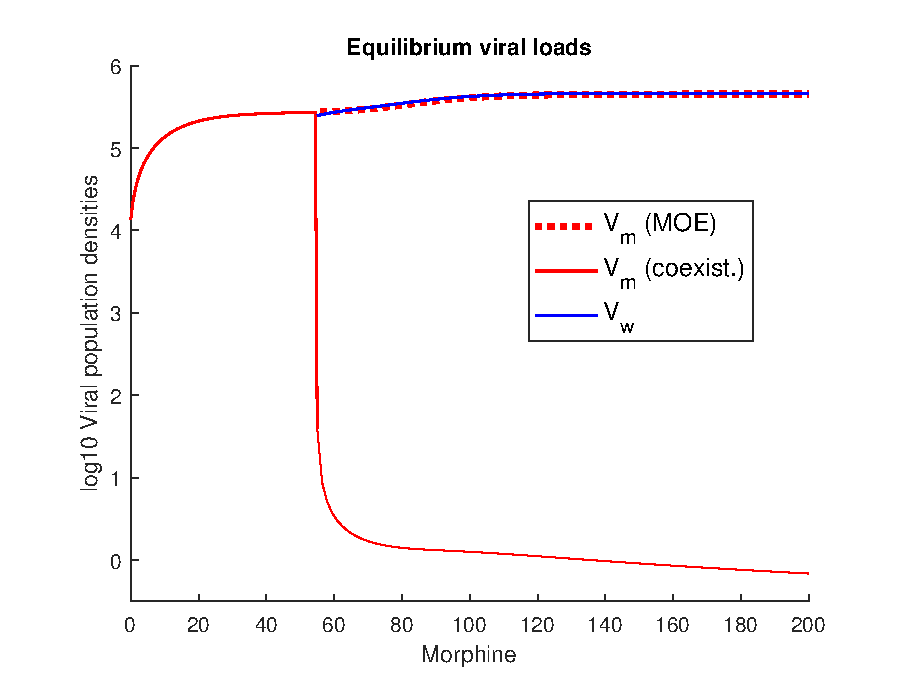
\includegraphics[scale=0.75]{equil_viral_loads_compared.eps}
\caption{Viral loads of the mutant only and coexistence equilibria. For $M<M_{thresh}$ the viral loads are the same, for  $M > M_{thresh}$ the viral load is mostly wild-type virus with a small amount of mutant.}
\label{fig:eq_vload}
\end{center}
\end{figure}

\begin{figure}[h]
\begin{center}
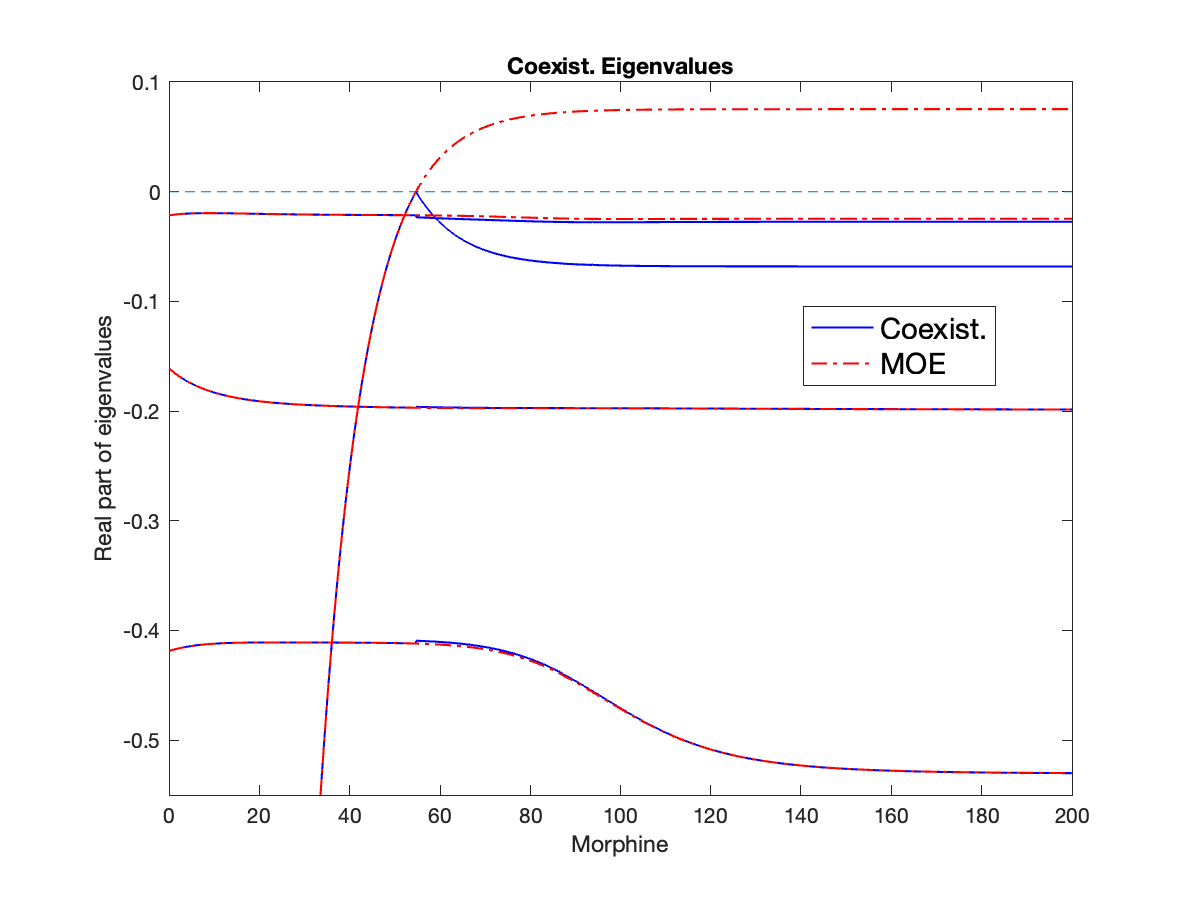
\includegraphics[scale=0.75]{coex_eigenvs.eps}
\caption{Real parts of eigenvalues of $J$ for the mutant only and coexistence equilibria. The eigenvalues separate at $M=M_{thresh}$, where the two equilibria separate and the MOE becomes unstable.}
\label{fig:coex_eig}
\end{center}
\end{figure}

In summary, the long-term dynamics of the model can be explained in terms of three biologically-relevant equilibria: the IFE, the MOE, and the coexistence equilibrium. Which of these the system arrives at is determined by $i)$ the strength of the mutant virus (in terms of the parameters $F$ and $B$) and $ii)$ the morphine concentration, $M$. A weak mutant virus (i.e. low $B$, high $F$) will fail to establish infection in the case of low morphine, while a high morphine concentration (i.e. $M>M_{thresh}$) will allow the wild-type virus to dominate with a small mutant population resulting from mutation. 

%\begin{figure}[h]
%%\begin{center}
%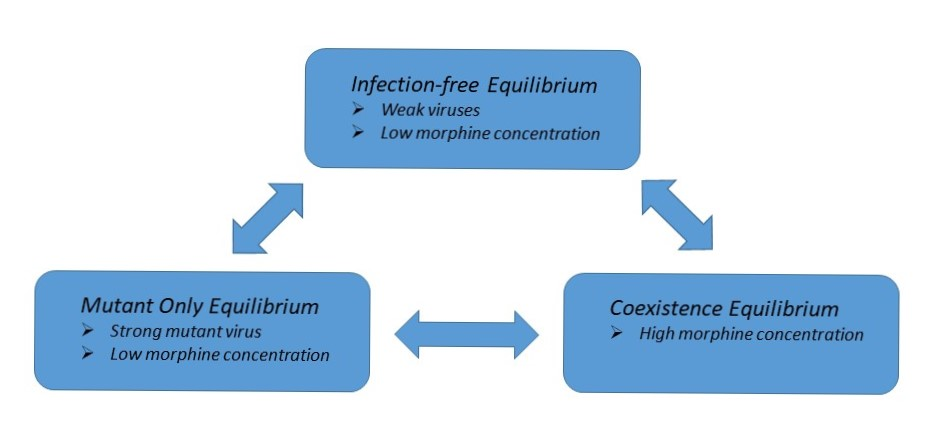
\includegraphics[scale=0.6]{cartoon.jpg}
%\caption{Cartoon of possible long-term outcomes of the model.}
%\label{fig:cartoon}
%%\end{center}
%\end{figure}

\subsection{Viral Load Simulations}

We can investigate the viral dynamics by solving the model numerically, with our interest primarily in the effects of morphine on the set-point viral load and its composition in terms of wild-type and mutant virus. Since $R_0 > 1$ for our base parameter values, we expect infection to be established for any concentrations of morphine. Figure~\ref{fig:base_sim}shows a one log increase in viral load for the case $M=200$ compared to $M=0$, similar to results found experimentally \cite{Kumar}.

\vspace{5mm}

\begin{figure}[h]
\begin{center}
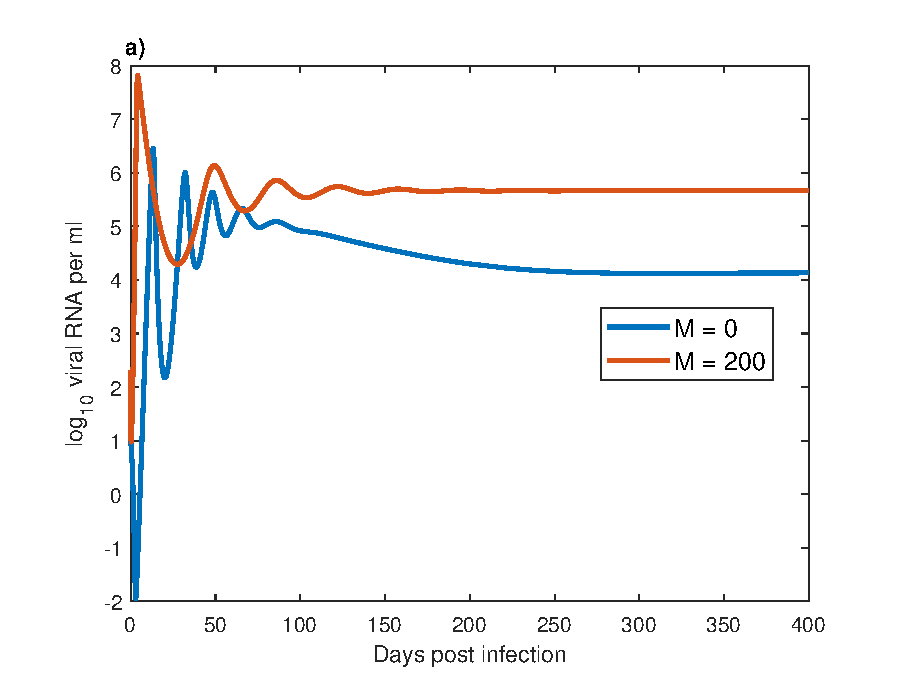
\includegraphics[scale=0.75]{base_sim.eps}
\caption{Predicted viral load for 200 days post-infection. $M=200$ results in a set-point viral load one log higher than $M=0$.}
\label{fig:base_sim}
\end{center}
\end{figure}

In Figure~\ref{fig:indv_sim}, we plot the viral loads of the wild-type and mutant viruses separately. For $M=0$, the viral load consists entirely of the mutant population with the wild-type population going extinct. When $M=200$, the wild-type population is dominate and makes up most of the viral load with a small, but positive steady-state amount of mutant virus. 

\vspace{5mm}

\begin{figure*}[h]
    \centering
    \begin{subfigure}[b]{0.5\textwidth}
        \centering
        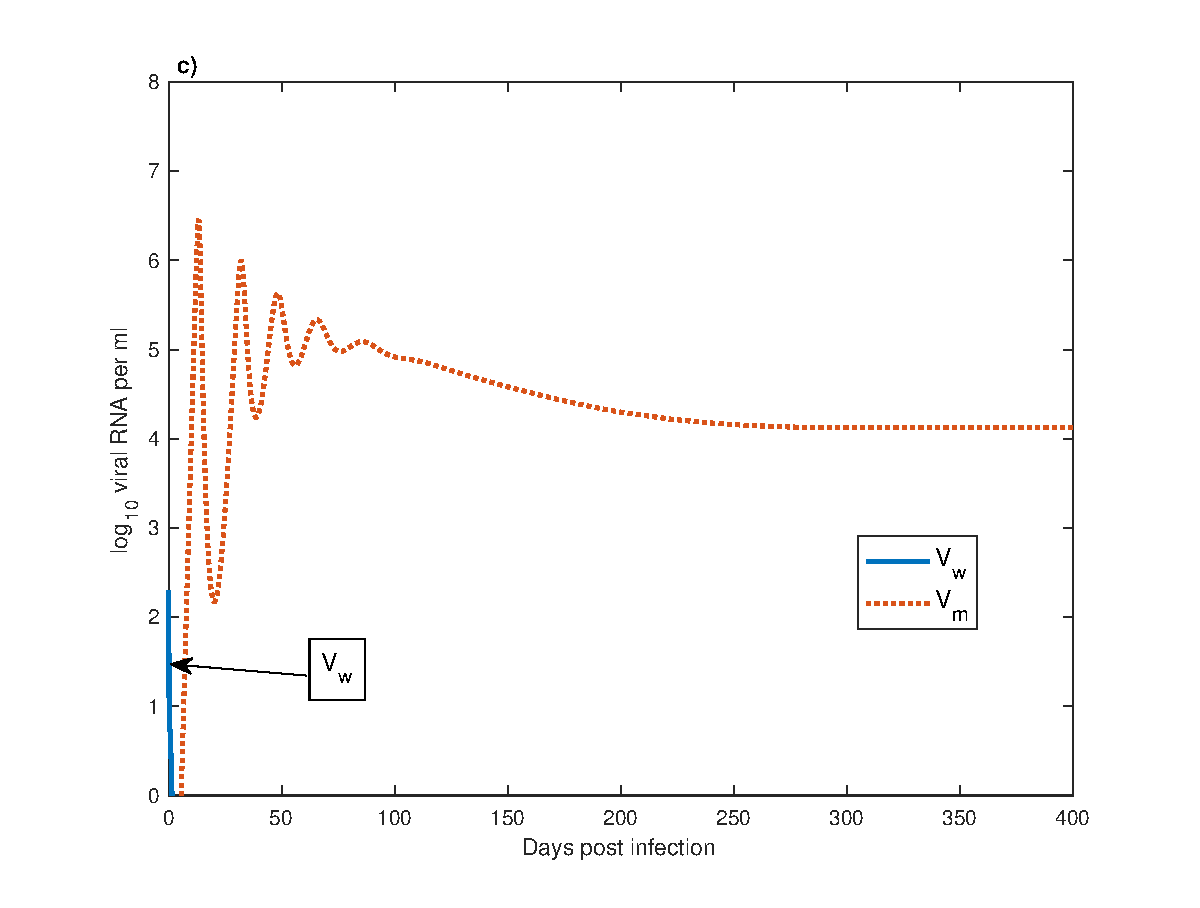
\includegraphics[scale=0.55]{ind_no_M.eps}
        %\caption{$R_w^0$ sensitivity indices}
    \end{subfigure}%
    ~ 
    \begin{subfigure}[b]{0.5\textwidth}
        \centering
        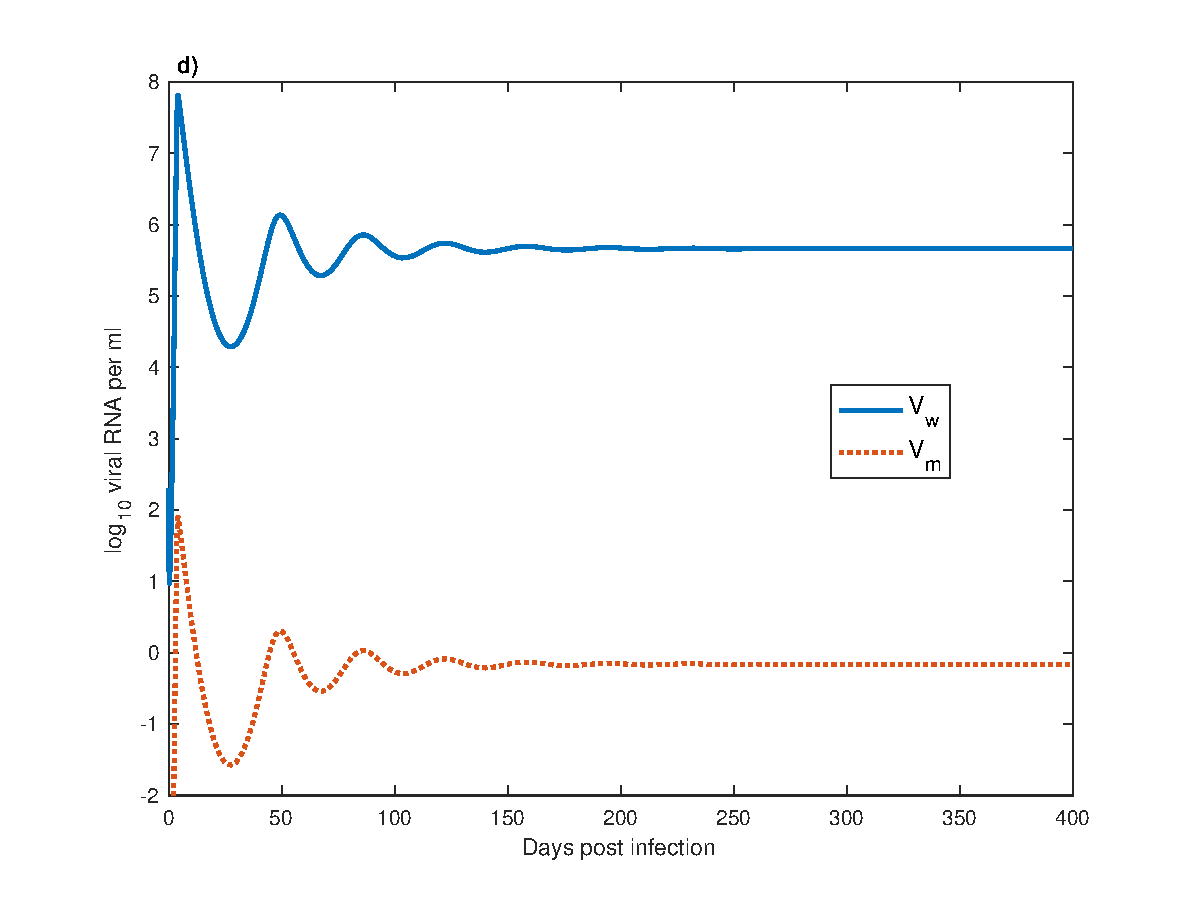
\includegraphics[scale=0.55]{ind_with_M.eps}
        %\caption{$R_w^0$ sensitivity indices}
    \end{subfigure}
    \caption{Individual viral populations for $M=0$ (left) and $M=200$ (right). For $M=0$, the wild-type virus goes extinct and the mutant is the dominant population. For $M=200$, the wild-type populations is dominant but a small amount of mutant virus persists due to mutation.}
\label{fig:indv_sim}
\end{figure*}

\section{Discussion}

HIV is an ongoing public heath problem around the world, and recreational use of injection drugs is one of the main risk factors for contracting it \cite{Alcabes}. In addition to increasing the risk of contracting HIV, injection drug use has been shown to have a number of adverse effects in such as a faster progression to AIDS, a higher chance of HIV related neurological complications, and an increased viral load \cite{Kumar,Hauser}. In this study, we present a mathematical model of HIV dynamics to investigate the effect of drugs of abuse (morphine) on viral load, immune effects, and viral evolution. We analyzed our model to determine the long-term outcome of an infection based on the concentration of morphine present and the fitness of the viral strain and determined conditions for each of the possible outcomes.

\vspace{5mm}

	We identified three biologically-relevant equilbria of the model and determined the locally stability of each. The infection-free equilibrium (IFE) is the solution of the model in which there are no infected components, i.e., no free virus or infected cells. The stability of the IFE is determined by the basic reproduction number, $R_0$, of the infection, with $R_0$ defined as the greater of the quantities $R_0^w$ and $R_0^m$ corresponding the to wild-type and mutant viruses, respectively \cite{Castillo-Chavez}. We calculated $R_0$ using the next-generation operator of the model, and found that $R_0^w$ and $R_0^m$ are increasing functions of morphine, indicating that both viral populations are more effective when morphine is present. In the case of no morphine, infection is established by the mutant virus and wild-type virus goes extinct. However, in the case of a less-fit mutant (determined by the fitness cost of mutation and mutant escape ratio), the IFE can become stable if $R_0^m < 1$.

\vspace{5mm}

	The mutant only equilibrium (MOE) is the steady-state solution of the model in which the wild-type virus has gone extinct and the viral load is composed entirely of mutant virus. We determined the local stability of this equilibrium by calculating the eigenvalues of the Jacobian matrix at the MOE. In the case where $R_0^m < 1$, the MOE and IFE represent the same equilibrium in which the infection has not been established. As $R_0^m$ passes through $1$ a bifurcation takes place the the MOE and IFE separate, the IFE becomes unstable, and the MOE remains stable. By calculating the eigenvalues of the Jacobian matrix as functions of morphine we determined that the MOE is stable only for low concentrations of morphine. 

\vspace{5mm}

	For a sufficiently high morphine concentration, both the MOE and IFE will be locally unstable and the dynamics will evolve to an equilibrium in which the viral load is almost entirely the wild-type virus but a small amount of mutant is produced via mutation. In this coexistence equilibrium, the reduced evolution caused by morphine prohibits the mutant virus from maintaining a significant population. In addition, the presence of morphine diminishes the cellular immune response by reducing the production rates of CTLs. Morphine also increases co-receptor expression in target cells, causing them to be more susceptible to infection. Combined with the higher infectivity of the wild-type virus, our model predicts a higher viral load when more morphine is present. If we take the fitness cost of mutation, $F$, and escape ratio, $B$, as control parameters then the model can predict the long-term out come of infection. The mutant virus is more likely to establish infection with a low value fitness cost and high escape ratio, and if $R_0^w, R_0^m < 1$ then the system will evolve to the infection-free equilibrium. If $R_0^m >1$ and $R_0^m > 1$ (where $R_0^m$ is a function of $F,B,$ and $M$) the system will evolve to the mutant only equilibrium.   

\vspace{5mm}

	Our model has several short-comings due to simplifying assumptions we made. Morphine is metabolized by the body and has decreasing concentration over time \cite{Olkkola}. Since we are primarily interested in the long-term outcome of infection, we assume a constant morphine concentration, $M$, and use this value in the analysis of the model- future work will focus on the dynamics with a time dependent morphine concentration. Many of the parameters are time dependent or morphine dependent in a way that is not captured in the model. Ganusov et al \cite{Ganusov2006, Ganusov2011} determined that the mutant escape from CTLs decreases over the course of infection. Vaidya et al \cite{Vaidya} parameterized their model to morphine-addicted and control rhesus macaques and found different parameter values between the two groups, here we largely used the control group parameters and allowed certain parameters to be morphine dependent (the transition rates between target cell groups, HIV evolution rate, and CTL production rates). 

\vspace{5mm}

	In summary, this study focuses on the long-term viral load of HIV and how it is affected by drug use. We found that morphine increases the viral load by weakening the host's cellular immune response, increasing the infectivity of the virus, and allowing the more infectious founding virus to dominate the viral dynamics. These results are further evidence that drug use is a serious obstacle to treating HIV. 


\pagebreak

\begin{thebibliography}{99}
\itemsep 0pt\relax

\bibitem{unaids}
UNAIDS. UNAIDS Data 2018 (2018) (find out how to cite this). %page 20

\bibitem{Alcabes}
P. Alcabes and G. Friedland, {\em Clinical Infections Diseases}, Clin. Infect. Dis. vol. 20, No. 6 (Jun., 1995), pp. 1467-1479.

\bibitem{Kohli}
R. Kohli, Y. Lo, A. A. Howard, D. Buono, M. Floris-Moore, R. S. Klein, and E. E. Schoenbaum, {\em Mortality in an Urban Cohort of HIV-Infected and At-Risk Drug Users in the Era of Highly Active Antiretroviral Therapy}, Clin. Infect. Dis. , vol. 41, No. 6 (Sep. 15, 2005), pp. 864-872.

%\bibitem{MMWR}
%{\em Morbidity and motality weekly report}. vol. 59 (2010) pp. 1550-1555.
%Morbidity and Mortality Weekly Report. Vol 59, No 47 (December 3, 2010), pp 1550-1555

\bibitem{Kumar}
R. Kumar, C. Torres, Y. Yamamura, I. Rodriguez, M. Martinez, S. Staprans, R. M. Donahoe, E. Kraiselburd, E. B. Stephens, and A. Kumar,  {\em Modulation by morphine of viral set point in rhesus macaques infected with simian immunodeficiency virus and simian-human immunodeficiency virus}, J. Virol. vol. 78 (2004) pp. 11425-11428.

\bibitem{Hauser}
K. F. Hauser, Y. K. Hahn, V. V. Adjan, S. Zou, S. K. Buch, A. Nath, A. J. Bruce-Kelle, and P. E. Knapp, {\em HIV-1 tat and morphine have interactive effects on oligodendrocyte survival and morphology},  Glia vol.  57 (2009) pp. 194-206. doi:10.1002/glia.20746.

\bibitem{Greenough}
T. C. Greenough, D. B. Brettler, M. Somasundaran, D. L. Panicali and J. L. Sullivan,  {\em Human immunodeficiency virus type 1- specific cytotoxic T lymphocytes (CTL), virus load, and CD4 T cell loss: evidence supporting a protective role for CTL in vivo}, J. Infect. Dis. vol. 176 (1997) pp. 118-125.

\bibitem{Klein}
M. R. Klein, S. H. van der Burg, O. Pontesilli, and F. Miedema, {\em Cytotoxic T lymphocytes in HIV-1 infection: a killing paradox?}, Immun. Today, vol. 19, no. 317, July 1998.

\bibitem{Fryer}
H. R. Fryer, J. Frater, A. Duda, M. G. Roberts, The SPARTAC Trial Inverstigators, R. E. Phillips, and A. R. McLean, {\em Modelling the Evolution and Spread of HIV Immune Escape Mutants}, PloS Pathogens, vol. 6, issue 11, November 2010.

\bibitem{Boutwell}
C. L. Boutwell, M. M. Rolland, J. T. Herbeck, J. I. Mullins, and T. M. Allen,  {\em Viral evolutions and escape during acute HIV-1 infection}, J. Infect. Dis. vol. 202 (2010) pp. S309-S314.

\bibitem{Perelson}
A. S. Perelson and  R. M. Ribeiro, {\em Modeling the within-host dynamics of HIV infection}, BMC Biol. (2013) http://www.biomedcentral.com/1741-7007/11/96

\bibitem{Chubb}
M. C. Chubb and K. H. Jacobsen,  {\em Mathematical modeling and the epidemiological research process}, Eur. J. Epidemiol. vol. 25 (2010) pp. 13-19.

\bibitem{Kitchen}
S. G. Kitchen, J. K. Whitmire, N. R. Jones, Z. Galic, C. M. R. Kitchen, R. Ahmed, J. A. Zack, and F. V. Chisari,  {\em The CD4 molecule on CD8+ T lymphocytes directly enhances the immune response to viral and cellular anitgens}, Proc. Natl. Acad. Sci. U.S.A. vol. 102 (2005) pp. 3794-3799.

\bibitem{Killeen}
N. Kileen, C. B. Davis, K. Chu, M. E. C. Crooks, S. Sawada, J. D. Scarborough, K. A. Boyd, S. G. Stuart, H. Xu, and D. R. Littman, {\em CD4 function in thymocyte differentiation and T cell activation}, Philos. Trans. R. Soc. Lond., B, Biol. Sci. vol. 342 (1993) pp. 25-34.

\bibitem{Chan}
D. C. Chan and P. S. Kim, {\em HIV entry and its inhibition}, Cell. vol. 93 (1998) pp. 681-684.

\bibitem{Fauci}
A. S. Fauci, {\em Pathogensis of HIV disease: Opportunities for new prevention interventions}, Clin. Infect. Dis. vol. 45 (2007) pp. S206-S212.

\bibitem{McMichael}
A. J. McMichael and S. L. Rowland-Jones, {\em Cellular immune responses to HIV}, Nature vol. 410 (2001) pp. 980-987.

\bibitem{Deng}
L. Deng, M. Pertea, A. Rongvauz, L. Want, C. M. Durand, G. Ghiaur, J. Lai, H. L. McHugh, H. Hao, J. B. Margolick, C. Gurer, A. J. Murphy, D. M. Valenzuela, G. D. Yancopoulus, S. G. Deeks, T. Stowig, P. Kumar, J. D. Siliciano, S. L. Salzberg, R. A. Flavell, L. Shan, and R. F. Siliciano, {\em Broad CTL response is required to clear latent HIV-1 due to dominance of escape mutations}, Nature vol. 517 (2015) pp. 381-385.

\bibitem{Ribeiro}
R. M. Ribeiro, L. L. Chavez, D. Li, S. G. Self, and A. S. Perelson, {\em Estimation of the initial viral growth rate and basic reproductive number during acute HIV-1 infection}, J. Virol. vol. 84 (2010) pp. 6096-6102.

%\bibitem{Ganusov2013}
%V. V. Ganusov, R. A. Neher, and A. S. Perelson, {\em Mathematical modeling of escape of HIV from cytotoxic T lymphocyte responses}, J. Stat. Mech. P01010-.foi:10.1088/1742-5468/2013/01/P01010.

%\bibitem{Ganusov2}
%V. V. Ganusov and R. J. De Boer, {\em Estimating costs and benefits of CTL escape mutations in SIV/HIV infection}, PloS Comput. Biol.(2006) https://doi.org/10.1371/journal.pcbi.0020024

\bibitem{Miyagi}
Miyagi, T., L. F. Chuang, R. H. Doi, M. P. carlos, J. V. Torres, and R. Y. Chuang. 2000. {\em Morphine induces gene expression of antiviral CCR5 in human CEMx174 lymphocytes}. J. Biol. chem. 275:31305-31310.

\bibitem{Li}
Y. Li, X. Wang, S. Tian, C. Guo, S. D. Douglas, and W. Ho, {\em Methadone enhances human immunodeficiency virus infection of human immune cells}, J. Infect. Dis. vol. 185 (2002) pp. 118-122.

\bibitem{Noel2006}
R. Noel, Z. Marrero-Otero, R. Kumar, G. S. Chompre-Gonzalez, A. S. Verma, and A, Kumar,  {\em Correlation between SIV tat evolution and AIDS progression in cerebrospinal fluid of morphine-dependent and control macaques infected with SIV and SHIV}, Virology vol. 349 (2006) pp. 440-452.

\bibitem{Noel2007}
R. Noel and A. Kumar, {\em SIV vpr evolution is inversely related to disease progression in a morphine-dependent rhesus macaque model of AIDS}, Virology vol. 359 (2007) pp. 397-404.

\bibitem{Rivera-Amill}
V. Rivera-Amill, P. S. Silverstein, R. Noel, S. Kumar, and A. Kumar,  {\em Morphine and rapid disease progression in nonhuman primate model of AIDS: Inverse correlation between disease progression and virus evolution}, J. Neuroimmune Pharmacol vol. 5 (2014) pp. 122-132. http://doi.org/10.1007/s11481-009-9184-0

\bibitem{Konrad}
B. P. Konrad, N. K. Vaiyda, and R. J. Smith?, {\em Modeling mutation to a cytotoxic T-lymphocyte HIV vaccine}, Math. Popul. Stud. vol. 18 (2011) pp. 122-149.

\bibitem{Conway}
J. M. Conway and A. S. Perelson, {\em Post-treatment control of HIV infection}, PNAS, vol. 112, no. 17, 5467-5472, April, 2015.

\bibitem{Schwartz}
E. S. Schwartz, K. R. H. Biggs, C. Bailes, K. A. Ferolito, and N. K. Vaidya, {\em HIV dynamics with immune responses: Perspectives from mathematical modeling}, Curr. Clin. Microbiol. Rep. vol. 3 (2016) pp. 216-224.

\bibitem{Vaidya}
N. K. Vaidya, R. M. Ribeiro, A. S. Perelson, and A. Kumar,  {\em Modeling the effects of morphine on simian immunodeficiency virus dynamics}, PloS Comput. Biol. (2016) https://doi.org/10.1371/journal.pcbi.1005127

\bibitem{Mutua}
J. M. Mutua, A.S. Perelson, A. Kumar, N. K. Vaidya, {\em Modeling the Effects of Morphine Altered Virus Specific Antibody Responses on HIV/SIV Dynamics}, Sci. Rep (2019) 9:5423.

\bibitem{Castillo-Chavez}
C. Castillo-Chavez, Z. Feng, and W. Huang,  {\em On the computation of $R_0$ and its role on global stability}, Mathematical Approaches for Emerging and Reemergin Infections Diseases: An Introduction, Springer-Verlag, New York, 2002, pp. 229-250.

\bibitem{Olkkola}
K. T. Olkkola, E. Maunuksela, R. Korpela, and P. H. Rosenberg,  {\em Kinetics and dynamics of postperative intravenous morphine in children}, Clin. Pharmacol. Ther. vol. 44 (1988) pp. 128-136.

\bibitem{Perko}
L. Perko, {\em Differential equations and dynamical systems}, 2nd ed., Springer-Verlag, New York, 1991.

\bibitem{Jordan}
D. W. Jordan and P. Smith,  {\em Nonlinear ordinary differential equations: An introduction to dynamical systems}, 3rd ed. Oxford University Press, New York, 1999.

\bibitem{Ganusov2006}
V. V. Ganusov and R. J. De Boer, {\em Estimating costs and benefits of CTL escape mutations in SIV/HIV infection}, PloS Comput. Biol.(2006) https://doi.org/10.1371/journal.pcbi.0020024

\bibitem{Ganusov2011}
V. V. Ganusov, N. Goonetilleke, M. K. P. Liu, G. Ferrari, G. M. Shaw, A. J. McMichael, P. Borrow, B. T. Korber, and A. S. Perelson, {\em Fitness Costs and Diversity of the Cytotoxic T Lymphocyte (CTL) Response Determine the Rate of CTL Escape during Acute and Chronic Phases of HIV Infection}, J. Virol. vol. 85 (2011) pp. 10518-10528.

\bibitem{Ganusov2013}
V. V. Ganusov, R. A. Neher, and A. S. Perelson, {\em Mathematical modeling of escape of HIV from cytotoxic T lymphocyte responses}, J. Stat. Mech. P01010-.foi:10.1088/1742-5468/2013/01/P01010.

\bibitem{Smith}
R. J. Smith and L. M. Wahl,  {\em Drug resistance in an immunological model of HIV-1 infection with impulsive drug effects}, Bull. Math. Biol. vol. 67 (2005) pp. 783-813.

\bibitem{Barouch}
D. H. Barouch, J. Kunstman, J. Glowczwskie, K. J. Kunstman, M. A. Egan, F. W. Peyerl, S. Santra, M. J. Kuroda, J. E. Schmitz, K. Beaudry, G. R. Krivulka, M. A. Lifton, D. A. Gorgon, S. M. Wolinsky, and N. L. Letvin,  {\em Viral escape from dominant simian immunodeficiency virus epitope-specific cytotoxic T lymphocytes in DNA-caccinated rhesus monkeys}, J. Virol. vol. 77 (2003) pp. 7367-7375.

\bibitem{Ramratnam}
B. Ramratnam, S. Bonhoeffer, J. Binley, A. Hurley, L. Zhang, J. E. Mittler, M. Markowitz, J. P. Moore, A. S. Perelson, and D. D. Ho, {\em Rapid production and clearance of HIV-1 and hepatitis C virus assessed by large volume plasma apheresis}, Lancet. vol. 354 (1999) pp. 1782.

\bibitem{Stafford}
M. A. Stafford, L. Corey, Y. Cao, E. S. Daar, D. D. Ho, and A. S. Perelson,  {\em Modeling plasma virus concentration during primary HIV infection}, J. Theor. Biol. vol. 203 (2000) pp. 285-301.

\bibitem{Mansky}
L. M. Mansky and H. M. Temin, {\em Lower in vivo mutation rate of human immunodeficiency virus type 1 than that predicted from the fidelity of purified reverse transcriptase}, J. Virol. vol. 69 (1995) pp. 5087-5094.

\bibitem{Marino}
S. Marino, I. B. Hogue, C. J. Ray, and D. E. Kirschner,  {\em A methodology for performing global uncertainty and sensitivity analysis in systems biology}, J. Theor. Biol. vol. 254 (2008) pp. 178-196.

\bibitem{De Boer}
R. J. De Boer and A. S. Perelson, {\em Target cell limited and immune control models of HIV jnfection: A comparison}, J. Theor. Biol. vol. 190 (1998) pp. 201-214.

\bibitem{Diekmann}
O. Diekmann, J. A. P. Heesterbeek, and M. G. Roberts, {\em The construction of next-generation matrices for compartmental epidemic models}, J. R. Soc. Interface (2009) http://rsif.royalsocietypublishing.org/content/7/47/873

\bibitem{Perera}
S. D. Perera, S. S. N. Perera, and S. Jayasinghe, {\em Modeling and sensitivity of dengue viral dynamics}, Int. J. Curr. Res. vol. 8 (2006) pp. 34899-34906.

\bibitem{Rodrigues}
H. S. Rodrigues, M. T. T. Monteiro, and D. F. M. Torres, {\em Sensitivity analysis in a dengue epidemiological model}, Conference Papers in Mathematics vol. 2013 (2013).

%\bibitem{Ganusov2011}
%V. V. Ganusov, N. Goonetilleke, M. K. P. Liu, G. Ferrari, G. M. Shaw, A. J. McMichael, P. Borrow, B. T. Korber, and A. S. Perelson, {\em Fitness Costs and Diversity of the Cytotoxic T Lymphocyte (CTL) Response Determine the Rate of CTL Escape during Acute and Chronic Phases of HIV Infection}, J. Virol. vol. 85 (2011) pp. 10518-10528.





\end{thebibliography}






\end{document} 